\documentclass{ktu_phd_summary}

\usepackage{ktu_phd}


\usepackage{siunitx}
\usepackage{array}

\usepackage{algorithm}
\usepackage{algorithmic}

\usepackage{colortbl}

\usepackage{array}
\newcommand{\PreserveBackslash}[1]{\let\temp=\\#1\let\\=\temp}
\newcolumntype{C}[1]{>{\PreserveBackslash\centering}p{#1}}
\newcolumntype{R}[1]{>{\PreserveBackslash\raggedleft}p{#1}}
\newcolumntype{L}[1]{>{\PreserveBackslash\raggedright}p{#1}}

%\pagenumbering{gobble}
%\pagenumbering{arabic}



\begin{document}



\begin{titlepage}
  \begin{center}

  %  \vspace*{20pt}

    \begin{figure}[H]
      \centering
    \scalebox{1.0}{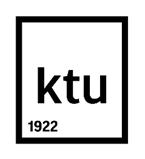
\includegraphics{images/NNwo6U.png}}
    \end{figure}

    \vspace*{30pt}

    \fontXII
    \textbf{Kauno technologijos universitetas}\\
    Matematikos ir gamtos mokslų fakultetas

    \vspace*{100pt}

    \fontXVIII
	   \textbf{Rekurentinio neuroninio tinklo apmokymas panaudojant grafinį vaizdo procesorių ir tinklo pritaikymas labiausiai tikėtinų žodžių pasiūlymui duotai sakinio pradžiai}\\
     \fontXIV
     Baigiamasis bakalauro projektas

     \vspace*{76.8pt}

     \fontXII

     % \begin{center}
     \singlespacing
     \begin{table}[H]
       \centering
      \begin{tabular}{C{90mm}}
      \arrayrulecolor[rgb]{0.831,0.686,0.216}\hline
       \\
      \begin{tabular}{@{}c@{}}\textbf{Deividas Riabčinskis}\\Projekto autorius\end{tabular} \\
       \\
      \begin{tabular}{@{}c@{}}\textbf{asist. Mindaugas Bražėnas}\\Vadovas\end{tabular} \\
       \\
        \begin{tabular}{@{}c@{}}\textbf{doc. Agnė Paulauskaitė-Tarasevičienė}\\Vadovė\end{tabular} \\
       \\ \arrayrulecolor[rgb]{0.831,0.686,0.216}\hline
      \end{tabular}
    \end{table}

\onehalfspacing

     \vfill

     \textbf{2019, Kaunas}

   \end{center}
\end{titlepage}



\begin{titlepage}
  \begin{center}

  %  \vspace*{20pt}

    \begin{figure}[H]
      \centering
    \scalebox{1.0}{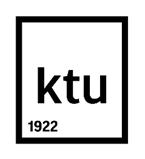
\includegraphics{images/NNwo6U.png}}
    \end{figure}

    \vspace*{30pt}

    \fontXII
    \textbf{Kauno technologijos universitetas}\\
    Matematikos ir gamtos mokslų fakultetas\\
    Informatikos fakultetas

    \vspace*{80pt}

    \fontXVIII
	   \textbf{Rekurentinio neuroninio tinklo apmokymas panaudojant grafinį vaizdo procesorių ir tinklo pritaikymas labiausiai tikėtinų žodžių pasiūlymui duotai sakinio pradžiai}\\
     \fontXIV
     Baigiamasis bakalauro projektas\\

     %\vspace*{55pt}
     \vspace*{40pt}

     \fontXII



     \singlespacing
     \hfill
     \begin{table}[H]
      \begin{tabular}{@{}L{85mm}@{}@{}L{85mm}@{}}
      \arrayrulecolor[rgb]{0.831,0.686,0.216}\hline
      &  \\
      \begin{tabular}{@{}l@{}}\textbf{Deividas Riabčinskis}\\Projekto autorius\end{tabular} &  \\
      &  \\
      \arrayrulecolor[rgb]{0.831,0.686,0.216}\hline
      &  \\
      \begin{tabular}{@{}l@{}}\textbf{Taikomoji matematika (612G10002)}\\\textbf{pagrindinės krypties studijos}\end{tabular} & \begin{tabular}{@{}l@{}}\textbf{Informatika (612I10004)}\\\textbf{gretutinės krypties studijos}\end{tabular} \\
      &  \\
      \arrayrulecolor[rgb]{0.831,0.686,0.216}\hline
      &  \\
      \begin{tabular}{@{}l@{}}\textbf{asist.}\\\textbf{Mindaugas Bražėnas}\\Vadovas\end{tabular} & \begin{tabular}{@{}l@{}}\textbf{doc.}\\\textbf{Agnė Paulauskaitė-Tarasevičienė}\\Vadovė\end{tabular} \\
      & \\
      \begin{tabular}{@{}l@{}}\textbf{lekt. dr.}\\\textbf{Mantas Landauskas}\\Recenzentas\end{tabular} & \begin{tabular}{@{}l@{}}\textbf{doc.}\\\textbf{Martynas Patašius}\\Recenzentas\end{tabular} \\
      & \\ \arrayrulecolor[rgb]{0.831,0.686,0.216}\hline
      \end{tabular}
    \end{table}

\onehalfspacing

     \vfill

     \textbf{2019, Kaunas}

   \end{center}
\end{titlepage}



\begin{titlepage}
  \begin{center}

  %  \vspace*{20pt}

    \begin{figure}[H]
      \centering
    \scalebox{1.0}{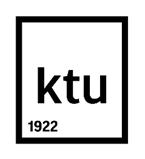
\includegraphics{images/NNwo6U.png}}
    \end{figure}

    \vspace*{30pt}

    \fontXII
    \textbf{Kauno technologijos universitetas}\\
    Matematikos ir gamtos mokslų fakultetas\\
    Deividas Riabčinskis

    \vspace*{100pt}

    \fontXVIII
	   \textbf{Rekurentinio neuroninio tinklo apmokymas panaudojant grafinį vaizdo procesorių ir tinklo pritaikymas labiausiai tikėtinų žodžių pasiūlymui duotai sakinio pradžiai}\\
     \fontXIV
     Akademinio sąžiningumo deklaracija

   \end{center}

     %\vspace*{55pt}
     \vspace*{40pt}

     \fontXII

     Patvirtinu, kad mano, Liepos Liepaitės, baigiamasis projektas tema „Baigiamojo projekto pavadinimas“ yra parašytas visiškai savarankiškai ir visi pateikti duomenys ar tyrimų rezultatai yra teisingi ir gauti sąžiningai. Šiame darbe nei viena dalis nėra plagijuota nuo jokių spausdintinių ar internetinių šaltinių, visos kitų šaltinių tiesioginės ir netiesioginės citatos nurodytos literatūros nuorodose. Įstatymų nenumatytų piniginių sumų už šį darbą niekam nesu mokėjęs.

     Aš suprantu, kad išaiškėjus nesąžiningumo faktui, man bus taikomos nuobaudos, remiantis Kauno technologijos universitete galiojančia tvarka.

\vspace*{40pt}

\begin{tabular}{@{}C{69.9mm}@{}@{}C{57.5mm}@{}@{}C{5.8mm}@{}@{}C{28.7mm}@{}@{}C{8mm}@{}}
  \hhline{~-~-~}
  \hhline{~-~-~}

& \textcolor{gray}{(vardą ir pavardę įrašyti ranka)} & & \textcolor{gray}{(parašas)} &
\end{tabular}


\end{titlepage}


\setcounter{page}{4}

Riabčinskis Deividas. Rekurentinio neuroninio tinklo apmokymas panaudojant grafinį vaizdo procesorių ir tinklo pritaikymas labiausiai tikėtinų žodžių pasiūlymui duotai sakinio pradžiai. Bakalauro baigiamasis projektas / vadovas Mindaugas Bražėnas; Kauno technologijos universitetas, Matematikos ir gamtos mokslų fakultetas.

Studijų kryptis ir sritis (studijų krypčių grupė): pagrindinų studijų - Taikomoji matematika (gamtos mokslai) ir gretutinių studijų Informatika (fiziniai mokslai), %(grupė mokslų nurodyti vėliau)

Kaunas 2019. %psl sk p.50

\begin{center}
\textbf{Santrauka}
\end{center}

Baigiamojo projekto darbo tikslas susidaryti ir išsivesti rekurentinio neuroninio tinklo vei\-ki\-mo formules ir tas formules realizuoti programiškai. Įvade aptariamas projekto aktualumas, suformuluojama problema ir iškeliami darbo uždaviniai. Literatūros analizės skyriuje nagrinėjami įvairūs neuroniai tinklai ir jų realizavimo metodai. LSTM rekurentinio tinklo skyriuje bus aprašytas tinklo veikimo principas, sudarytos ir išvestos formulės reikalingos tinklui apmokinti ir prognozuoti reikšmes.

\clearpage

Riabčinskis Deividas. Recurrent neural network training using GPU and its application for suggesting the most probable words given the beginning of sentence. Bachelor's Final Degree Project / Mindaugas Bražėnas; The Faculty of Mathematics and Natural Sciences, Kaunas University of Technology.


Kaunas, 2019. 48 p.

\begin{center}
\textbf{Summary}
\end{center}


\clearpage



% . Galios ir energijos matavimo mazgas lokaliam LED šviestuvui. Bakalauro baigiamasis projektas / vadovas prof. ; Kauno technologijos universitetas, Elektros ir elektronikos fakultetas.
% Studijų kryptis ir sritis (studijų krypčių grupė): Elektronikos ir elektros inžinerija, Technologijos mokslai (inžinerija).
% Reikšminiai žodžiai: galia, energija, matavimai, mikrovaldiklis.
% Kaunas 2019. 48 p.
% Santrauka
% Baigiamojo projekto darbo tikslas yra sukurti aparatinį ir programinį sprendimą LED šviestuvo suvartojamos galios ir energijos matavimui. Įvade aptariamas projekto aktualumas, suformuluojama problema ir iškeliami darbo uždaviniai.
% Problemos analizės skyriuje nagrinėjami iššūkiai, su kuriais susiduriama atliekant srovės ar įtampos matavimus, taip pat analizuojama srovės ir įtampos matavimų metodika siekiant pasirinkti tinkamiausią ir kokybiškiausią kainos atžvilgiu matavimo variantą.
% Tyrimų dalyje sudaromos matavimų grandžių simuliacijos, ištiriama komponentų nominalų bei jų tolerancijų reikšmė atliekant tikslumo reikalaujančius matavimus.
% Projektinės dalies skyriuje apžvelgiamos ir išanalizuojamos elektrinės schemos, suprojektuotos galios ir energijos matavimo prietaisui, atliekama papildomo tyrimo analizė suprojektuotam prietaisui, nuodugniai išnagrinėjami C programavimo kalbos pagrindu sudaryti programos algoritmai, taip pat pateikiami atliktų galios bei energijos matavimų tyrimų rezultatai, jų duomenų palyginimas su etaloniniu prietaisu.
%
% . Solution for power and energy measurement for local LED lamp. Bachelor's Final Degree Project / prof. ; Electrical and Electronics Faculty, Kaunas University of Technology.
% Study field and area (study field group): Electronics and Electrical Engineering, Technological sciences (Engineering).
% Keywords: power, energy, measurements, microcontroller.
% Kaunas, 2019. 48 p.
% Summary
% The aim of the final project work is to create a hardware and software solution for measuring the power and energy consumption of the LED luminaire. The introduction discusses the relevance of the project, formulates the problem and raises the tasks.
% The problem analysis section examines the challenges facing current or voltage measurements, analyzes the current and voltage measurement methodology to select the most appropriate and the best quality-price ratio measurement option.
% In the part of the researches the simulations of the measurement chains are made, the value of the component denominations and their tolerances in the measurements requiring accuracy are investigated.
% The project section reviews and analyzes the electrical schemes designed for the power and energy measuring device, the analysis of the additional research for the designed device, the program algorithms based on the C programming language are thoroughly analyzed, the results of the performed power and energy measurements as well as their data comparison with the reference device are presented.


%%
%% Table of contents & lists
%%
\tableofcontents
\clearpage

\listoffigures
\clearpage

% \listoftables
% \clearpage

\section*{Įvadas}
\addcontentsline{toc}{section}{Įvadas}
Šiais laikais labai daug yra kalbama apie dirbtinį intelektą, robotus, kurie jau dabar yra naudojami padedant žmonėm atlikti kasdienius darbus ir netgi robotai keičia žmones gamyklose atliekant specifinius darbus.

Šiuolaikinėje visuomėneje, turbūt nei vienas negali įsivaizduoti gyvenimo be telefono ar mašinos. Naudojant dirbtinį intelektą yra kuriamos telefoninės aplikacijos, kurios leidžia siųsti sms žinutes jų nerašant, o pasakant žinutės tekstą balsu, taip pat muzikinės aplikacijos, kurios padeda surasti dainos pavadinimą išgirdus melodijai ir netgi dirbtinis intelektas yra naudojamas kaip vertėjas, gali du žmonės šnekėti skirtingomis kalbomis, bet naudojant dirbtinį intelektą, žodžiai iškart yra išverčiami į gimtąją kalbą. Kompanijos TESLA yra kuriami automobiliai, kurie turi įrangą, kuri leidžia automobiliams patiems važiuoti.

Dirbtinis intelektas yra kuriamas naudojant visokiausius neuroninius tinklus. Šie tinklai veikia panašiai kaip žmogaus smegenys, kaip žmogaus smegenų ląstelės. Šių tinklų yra įvairiausių rūšių, nuo paprastų neuroninių tinklų iki rekurentinių neuroninių tinklų.

Projekto tikslas - sukurti neuroninį tinklą, kuris būtų galimas pritaikyti praktikoje. Mano tikslas šį tinklą pritaikyti taip, kad jis išmoktų pasiūlyti, žmogui rašančiam tekstą, pradėto rašyti žodžio galą ir sekantį žodį.

Darbo uždaviniai:

\begin{enumerate}
  \item (Pagrindinių studijų) Surasti informacijos apie rekurentinius neuroninius tinklus ir suprasti jų veikimą.
  \item (Pagrindinių studijų) Išsivesti rekurentinio neuroninio tinklo, LSTM (angl. \textit{Long Short Term Memory}) apmokymo formules.
  \item (Greutinių studijų) Formules realizuoti programiškai.
  \item (Greutinių studijų) Pritaikyti tinklą prognozuoti rašomo žodžio galą ir sekantį žodį.
  \item (Greutinių studijų) Optimizuoti tinklą.
  \item (Pagrindinių studijų) Atlikti suprogramuoto rekurentinio neuroninio tinklo veikimo analizę.
\end{enumerate}

\clearpage


\clearpage

\section{Literatūros apžvalga}
Čia yra literatūros apžvalga. Šitas mokslininkas padarė taip \cite{horvath2016}.
%
Kitas klausimas.

Toliau apžvelgsime \cite{ezhov1969} darbus.

https://machinelearningmastery.com/learning-rate-for-deep-learning-neural-networks/

Neuroniai tinklai arba kitaip dirbtinio intelekto neuroniai tinklai yra mašininio mokymo metodai, kurie leidžia kompiuteriui mokytis iš stebimų duomenų. Neuroninių tinklų veikimo principas yra įkvėptas pagal tai kaip biologinė nervų sistema apdoroja informaciją.\cite{Sukhadeve2017}

% Neuroninių tinklų sprendžiamos problemos

Esminis neuroninio tinklo elementas yra dirbtinis neuronas. Šį neuroną sudaro pagrindiniai trys komponentai: įvesties reikšmės, svoriai, kurie jungia šias reikšmes su neuronu ir aktyvacijos funkcija. Tai yra pats paprasčiausias neurono modelis, vadinamas Perceptronu (angl. \textit{Perceptron}).\cite{Andrew2017}

\begin{figure}
  \centering
\scalebox{0.5}{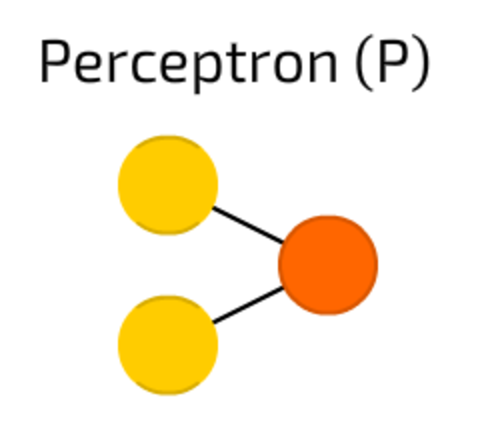
\includegraphics{images/perceptron.png}}
\caption{Testuojam jpg įtraukimą.}
\end{figure}

\begin{figure} \label{fig:perceptron}
  \centering
\scalebox{0.5}{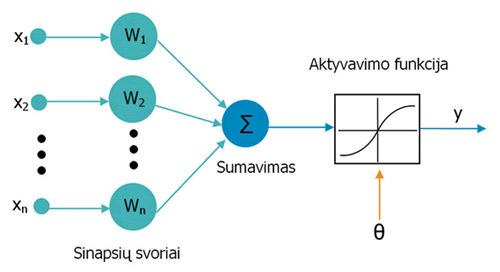
\includegraphics{images/perceptron_pvz.png}}
\caption{Dirbtinio neurono modelis (Perceptronas).}
\end{figure}

Paveiksle pavaizduoto Perceptrono reikšmė apskaičiuojama pagal formulę
\begin{equation*}
  y = f \left(\sum_{k=1}^{n} x_k W_k \right),
\end{equation*}

čia f - aktyvavimo funkcija.

Paveiksle \ref{fig:perceptron} pavaizduoto neurono veikimo principas:
\begin{enumerate}

\item Neuronas gauna įvesties reikšmes $x_1, x_2, ... , x_n$. Kiekviena iš reikšmių turi savo perdavimo koeficientą į neuroną (svorį) $W_1, W_2, ... , W_n$.
\item  Skaičiuojama įvesties reikšmių ir atitinkamų svorių sandaugų suma(žymima z):
  $z = \sum_{k=1}^{n} x_k * W_k$
\item  Neurono išvesties reikšmė(žymima a) yra apskaičiuojama įvesties reikšmių ir atitinkamų svorių sandaugų sumai pritaikius aktyvacijos funkciją(žymima f).
  $a = f(z) = f(\sum_{k=1}^{n} x_k * W_k)$
\end{enumerate}

\subsection{Sužadinimo signalai(angl. \textit{Bias neuron})}
Dažniausiai įvesties reikšmių yra vienetu daugiau, nei yra paduodama įvesties reikšmių. Ši įvestis yra vadinama sužadinimo signalu (angl. \textit{Bias neuron}). Šio signalo reikšmė yra pastovi ir visada lygi vienetui($x_{n+1} = 1$). Taip pat yra pridedamas papildomas svoris $W_{n+1}$ jungiantis šį signalą su neuronu.\cite{Ieva2012}
Šis sužadinimo signalas padeda lengvai koreguoti neurono išvesties reikšmę, kadangi įvesties reikšmė yra vienetas, tuomet sandauga, kuri yra prisumuojama priklauso tik nuo svorio jungiančio sužadinimo signalą su neuronu. Ji yra lygi  $W_{n+1}$. Naudojant sužadinimo signalus neuroniai tinklai yra daug sparčiau apmokinami, kadangi šie signalai gali laisvai koreguoti perduodamą reikšmę į neuronus.
  \subsection{Aktyvacijos funkcijos(angl. \textit{Activation function})}
Neurono išvesties reikšmei apskaičiuoti naudojamų aktyvacijos funkcijų yra visokiausių tipų.




Patys pirmieji neuroninio tinklo modeliai buvo sukurti Tiesioginio sklidimo (angl. \textit{Feed forward}) neuroniniai tinklai.

\cite{Ieva2012}


%padaryti feedforward vieno apskaiciavima
Šiuo būdu realizuoto neurononio tinklo schema pavaizduota (). Čia




\begin{figure}
  \centering
\scalebox{0.5}{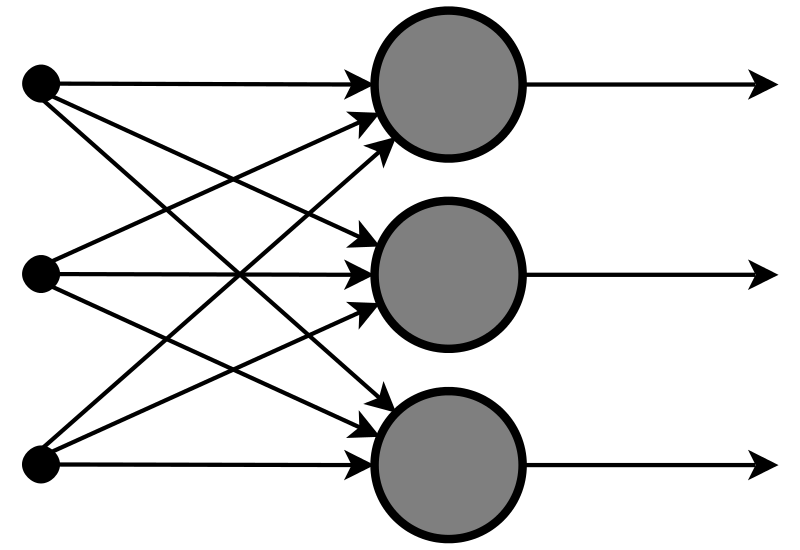
\includegraphics{images/feedforward.png}}
\caption{Testuojam jpg įtraukimą.}
\end{figure}



Dirbtinis intelektas


neuroniai tinklai, ju tipai


Neuroninių tinklų yra daug tipų, pagal



lstm neuroninis tinklas

taikymas language Modelling


Dirbtinis intelektas


\clearpage



\section{LSTM rekurentinis neuroninis tinklas}
Bendrai apie LSTM, jo 


% \subsection{Veikimo principai}
%sandara
Apžvelgsime rekurentinio neuroninio tinklo, LSTM (angl. \textit{Long Short Term Memory}), veikimo principus.
Rekurentinis neuroninis tinklas turi savyje atmintį(t.y. tinklas išvesdamas apskaičiuotas reikšmes atsižvelgia į tai kas vyko praeityje).

Rekurentiniai neuroniniai tinklai, kitaip, nei paprasti neuroniniai tinklai turi grįštamuosius ryšius. Tai reiškia, kad šie tinklai apskaičiuodami naujas tinklo išvesties reikšmes atsižvelgia į praeitį. Šiam tikslui pasiekti rekurentiniai neuroniai tinklai savyje turi atmintį, kuri priklauso nuo prieš tai, kas vyko praeityje. Taip pat šis tinklas kaip įvesties reikšmes priema ne tik esamame laiko žingsnyje esamas įvesties reikšmes, bet ir praeito žingsnio išvesties reikšmes(būsenas), kas dar labiau padeda tinklui prognozuoti išvesties reikšmes priklausomai nuo praeities reikšmių.

Šie rekurentiniai neuroniai tinklai savyje turi keturis paprastus neuroninius tinlus, kur kiekvienas iš jų atlieka savo paskirtį. Pirmasis neuroninis tinklas veikia, taip kad jo išvesties reikšmės nurodo kokią informaciją reikia pamiršti(t.y informaciją, kuri yra nereikšminga). Antrasis neuroninis tinklas kontroliuoja kiek naujos informacijos iš įvesties reikšmių reikia pridėti prie esamos informacijos. Trečiasis neuroninis tinklas dar papildomai pakoreguoja kiek naujos informacijos reikia išsisaugoti. Ketvirtasis neuroninis tinklas kontroliuoja kiek esamos informacijos turi būti perduodama apskaičiuojant naują tinklo išvesties reikšmę(būseną).

Reukurentinio neuroninio tinklo apmokymas vyksta į tinklą paduodant tam tikrus rinkinius duomenų. Tie rinkiniai sudaryti iš įvesties reikšmių ir reikšmių, kurias tikimasi gauti iš tinklo. Iš pradžių duomenys yra praleidžiami pro tinklą (angl. \textit{Feed forward}) ir poto atliekamas baudos funkcijos paklaidos mažinimas anti-gradientinio nusileidimo metodu (angl \textit{Back Propogation}).

Kiekvieno neuroninio tinklo sluoksnio neuronų kiekis yra vienetu didesnis, nei yra nurodyta tinklo topologijoje, dėl to, kad paskutinis atitinkamo sluoksnio neuronas yra pridedamas, kuris padeda greičiau apmokyti tinklą. Šis neuronas yra vadinamas "Bias" neuronu ir jo reikšmė visada yra lygi 1.

h\textss{(t)}

\begin{aligned}
  \begin{math}h_i^{(t)}\end{math} - vektorius, kuris saugo t laiko momentu gautas tinklo išvesties reikšmes.\\
  \begin{math}c_k^{(t)}\end{math} - vektorius, kuris saugo t laiko momentu gautas tinklo atminties reikšmes.\\
  \begin{math}M\end{math} - išvesties ir atminties vektorių ilgis.\\
  \begin{math}I\end{math} - įvesties reikšių vektoriaus ilgis.\\
  \begin{math}L\end{math} - nurodo kiek sluoksnių yra atitinkamame tinkle.\\
  \begin{math}l\end{math} - nurodo kiek neuronų yra atitinkamo tinklo l-ame sluoksnyje.\\
  \begin{math}w_{ij}^{(v,s)}\end{math} - nurodo v-ojo tinklo svorį iš s-ojo sluoksnio i-ojo neurono į (s+1)-ojo sluoksnio j-ąjį neuroną.\\
  \begin{math}a_k^{(u,l)}\end{math} - nurodo u-ojo tinklo, l-ojo sluoksnio, k-ojo neurono reikšmę.\\
  \begin{math}z_k^{(u,l)}\end{math} - nurodo u-ojo tinklo, l-ojo sluoksnio, k-ojo neurono sumą.\\
  \begin{math}K(u,l)\end{math} - nurodo u-ojo sluoksnio, l-ojo sluoksnio neuronų kiekį. \\
  \begin{math}b_k^{(t))}\end{math} - nurodo tarpines k-asias išvesties reikšmes.\\
  \begin{math}E^{(t)}\end{math} - tinklo baudos funkcija.\\
  \begin{math}\delta_{u,v}\end{math} - delta funkcija, kuri gražina vienetą, jei u sutampa su v. \\
  \begin{math}\end{math}
  \begin{math}\end{math}
\end{aligned}





\begin{equation}\label{eq:variables}
  h_k^{(t)} -
\end{equation}


\subsection{LSTM išvesties reikšmės apskaičiavimas}
Feed forward'as

\begin{equation} \label{eq:forward}
  \vec{a}_i = \sum_{k=0}^{M} \frac{\partial a_{k}^{(u,l)}}{\partial \mx{W}_{i,j}^{(v,s)}}
\end{equation}

\begin{equation*}
  \begin{aligned}
    \vec{a} = &\left( x^2 \right) = \\ % komentaras
    &b+\sqrt{c} + h + 1 \\
    a = \left \{
    \begin{aligned}
      &\text{kai } l=1 & d+f\\
      &\text{kai } l=2 & d+f+8
    \end{aligned}
    \right.
  \end{aligned}
\end{equation*}

Šitoje formulėje (\ref{eq:forward})


\subsection{LSTM apmokymas gradientinio nusileidimo metodu}
% Backpropagation metodas
% \mx{W}
Atliktus įvesties reikšmių perleidimą per tinklą yra skaičiuojamas baudos funkcijos reikšmė, kuri yra lygi vidutinei kvadratinei tinklo paklaidai. Jos formulė yra (\ref{eq:Ett}).

%
% \begin{equation*} \label{eq:Et}
%   \begin{aligned}
%     \vec{E} = &\left( x^2 \right) = \\ % komentaras
%     &b+\sqrt{c} + h + 1 \\
%     a^{(t)} = \left \{
%     \begin{aligned}
%       &\text{kai } l=1 & d+f\\
%       &\text{kai } l=2 & d+f+8
%     \end{aligned}
%     \right.
%   \end{aligned}
% \en{equation*}

\begin{equation} \label{eq:Ett}
  \begin{aligned}
  E^{(t)} = \sum_{k=1}^{M} \frac{1}{2}(y_k^{(t)} - h_k^{(t)})^{2},
  \end{aligned}
\end{equation}
čia $h_k^{(t)}$ - tinklo išvesties reikšmė, o $y_k^{(t)}$ - prognozuojama reikšmė, kurią turime gauti.

Apmokymo tikslas yra mažinti baudos funkcijos reikšmę, tam yra naudojamas gradientinio nusileidimo metodas. Šis metodas leidžia atnaujinti neuroninių tinklų svorius priešinga gradiento kryptimi, kas sumažina vidutinę tinklo išvesties reikšmių paklaidą.

 Svorių atnaujinimas vyksta skaičiuojant tinklo baudos funkcijos išvestinę pagal kiekvieną iš tinkle esančių svorių \ref{eq:E_deriv}. Atnaujinant svorius yra apskaičiuojamas ir saugomas $\Delta w_{ij}^{(u,l)}$. Jis yra apskaičiuojamas naudojant prieš tai buvusį svorio pokytį padauginus iš atitinkamos $\alpha$ reikšmės ir atėmus baudos funkcijos išvestinės reikšmę pagal atitinkamą svorį padaugintą iš $\eta$ (\ref{eq:weightupdate}). Šie $\alpha $ ir $\alpha$ parametrai nurodo mokymosi greitį. $\alpha$ - nurodo tinklo inertiškumą, tai yra kiek tinklo naujo svorio reikšmę priklauso nuo prieš tai buvusių svorių. $\eta$ - nurodo tinklo apmokymo greitį, tai yra kiek tinklo nauja svorio reikšmė priklauso nuo dabartiniu laiko momentu įvykdyto apmokymo.


\begin{equation}\label{eq:weightupdate}
  \Delta w_{ij}^{(u,l)} = -\eta\frac{\partial E^{(t)}}{\partial w_{ij}^{(u,l)}} + \alpha\Delta w_{ij}^{(u,l)},
\end{equation}
čia $\alpha$ - inercija, $\eta$ - apmokymo greitis.

Tada bendra svorio atnaujinimo gaunama formulė yra (\ref{eq:weightsupdate}) :

\begin{equation}\label{eq:weightsupdate}
  w_{ij}^{(u,l)} = w_{ij}^{(u,l)} + \Delta w_{ij}^{(u,l)}
\end{equation}

\begin{equation} \label{eq:E_deriv}
  \begin{aligned}
  \frac{\partial E^{(t)}}{\partial w_{ij}^{(v,s)}} = \sum_{n=1}^{M} \frac{\partial (\sum_{k=1}^{M} \frac{1}{2}(y_m^{(t)} - h_m^{(t)})^{2})}{\partial h_n^{(t)}} \frac{\partial h_n^{(t)}}{\partial w_{ij}^{(v,s)}},
  \end{aligned}
\end{equation}
čia $\frac{\partial h_k^{(t)}}{\partial w_{ij}^{(v,s)}}$ yra apskaičiuojama pagal formulę (\ref{eq:hn}).


\begin{equation} \label{eq:hn}
  \begin{aligned}
  \frac{\partial h_k^{(t)}}{\partial w_{ij}^{(v,s)}}
  =
  \sum_{n=1}^{M}
  \frac{\partial (\frac{e^{b_k^{(t)}}}{\sum_{m=1}^{M} e^{b_m^{(t)}}})}
  {\partial b_n^{(t)}}
   \frac{\partial b_n^{(t)}}{\partial w_{ij}^{(v,s)}},
   \end{aligned}
\end{equation}
čia $\frac{\partial b_n^{(t)}}{\partial w_{ij}^{(v,s)}}$ yra apskaičiuojama pagal formulę (\ref{eq:bn}).




\begin{equation} \label{eq:bn}
  \begin{aligned}
  \frac{\partial b_n^{(t)}}{\partial w_{ij}^{(v,s)}}
  =
  \frac{\partial (a_k^{(o,L)} tanh(c_k^{(t)}))}{\partial w_{ij}^{(v,s)}}
  =
  \frac{\partial a_k^{(o,L)}}{\partial w_{ij}^{(v,s)}} tanh(c_k^{(t)}) +
  a_k^{(o,L)} \frac{\partial tanh(c_k^{(t)})}{\partial w_{ij}^{(v,s)}},
  \end{aligned}
\end{equation}
čia išskiriam dvi išvestines $\frac{\partial a_k^{(o,L)}}{\partial w_{ij}^{(v,s)}}$ ir $\frac{\partial tanh(c_k^{(t)})}{\partial w_{ij}^{(v,s)}}$, kurios yra apskaičiuojamos pagal formules (\ref{eq:a_derivl-1}) ir (\ref{eq:tanh_deriv_byc}) atitinkamai.


\begin{equation} \label{eq:tanh_deriv_byc}
  \begin{aligned}
  \frac{\partial tanh(c_k^{(t)})}{\partial w_{ij}^{(v,s)}} =
  \frac{\partial tanh(c_k^{(t)})}{\partial c_k^{(t)}}
  \frac{\partial c_k^{(t)}}{\partial w_{ij}^{(v,s)}},
  \end{aligned}
\end{equation}
čia $\frac{\partial c_k^{(t)}}{\partial w_{ij}^{(v,s)}}$ yra apskaičiuojama pagal formulę (\ref{eq:c_deriv}).


\begin{equation} \label{eq:c_deriv}
  \begin{aligned}
    \frac{\partial c_k^{(t)}}{\partial w_{ij}^{(v,s)}} =&
      \frac{\partial (c_k^{(t-1)}a_k^{(f,L)}+a_k^{(i,L)}a_k^{(g,L)})}{\partial w_{ij}^{(v,s)}} =\\
  &\frac{ \partial c_k^{(t-1)}}{\partial w_{ij}^{(v,s)}}a_k^{(f,L)} +
  c_k^{(t-1)}\frac{\partial a_k^{(f,L)}}{\partial w_{ij}^{(v,s)}} +
  \frac{\partial a_k^{(i,L)}}{\partial w_{ij}^{(v,s)}}a_k^{(g,L)} +
  a_k^{(i,L)}\frac{\partial a_k^{(g,L)}}{\partial w_{ij}^{(v,s)}}
  \end{aligned}
\end{equation}

Toliau išvesime bendrąją $\frac{\partial a_k^{(u, l)}}{\partial w_{ij}^{(v,s)}}$ formulę, kuria būtų galima apskaičiuoti bet kurio tinklo $a_k^{(u, l)}$ reikšmės išvestinę pagal bet kurį $w_{ij}^{(v,s)}$ (\ref{eq:gkv}).

Norint tai atlikti iš pradžių reikia apskaičiuoti bet kurio tinklo paskutiniojo sluoksnio $a_k^{(u, L)}$ išvestinę pagal vienu žemiau esančio sluoksnio svorį $w_{ij}^{(v,L-1)}$ (\ref{eq:a_derivl-1}).

Pastaba! Tinklų išvesties reikšmės $a_k^{(u, l)}$ yra funkcijos, kurios priklauso nuo visų esančių tinklų svorių. Dėl šitos priežasties yra skaičiuojamos visų tinklų $a_k^{(u, l)}$ išvestinės, pagal visų tinklų svorius.

\begin{equation} \label{eq:a_derivl-1}
  \begin{aligned}
  \frac{\partial a_k^{(u, L)}}{\partial w_{ij}^{(v,L-1)}} =
  \frac{\partial f(z_k^{(u, L)})}{\partial w_{ij}^{(v,L-1)}} =
  \frac{\partial f(z_k^{(u, L)})}{\partial z_k^{(u,L)}} \frac{\partial z_k^{(u,L)}}{\partial w_{ij}^{(v,L-1)}},
  \end{aligned}
\end{equation}
čia u ir v - nurodo, kad tinklai, kuriose yra kintamieji $a_k^{(u, L)}$ ir $w_{ij}^{(v,L-1)}$ nebūtinai turi sutapti.

Toliau apskaičiuojame $\frac{\partial z_k^{(u,L)}}{\partial w_{ij}^{(v,L-2)}}$ (\ref{eq:z_deriv}).

\begin{equation} \label{eq:z_deriv}
  \begin{aligned}
    \frac{\partial z_k^{(u,L)}}{\partial w_{ij}^{(v,L-1)}} =& \sum_{n=1}^{K(u, L-1)+1}
      \frac{ \partial (\sum_{m=1}^{K(u,L-1)+1} w_{mk}^{(u,L-1)} a_m^{(u,L-1)} ) }{ \partial a_n^{(u,L-1)} }  \frac{\partial a_n^{(u,L-1)}}{\partial w_{ij}^{(v,L-1)}} + \\
      &\sum_{n=1}^{K(u, L-1)+1} \frac{\partial (\sum_{m=1}^{K(u,L-1)+1} w_{mk}^{(u,L-1)a_m^{(u,L-1)}} )}{\partial w_{nk}^{(v,L-1)}}
      \frac{\partial w_{nk}^{(v,L-1)}}{\partial w_{ij}^{(v,L-1)}} = \\
      &\sum_{n=1}^{K(u, L-1)+1} w_{nk}^{(u,L-1)}  \frac{\partial a_k^{(u, L-1)}}{\partial w_{ij}^{(v,L-1)}}  +  \frac{\partial f(z_k^{(u, L)})}{\partial z_k^{(u,L)}}  \delta_{u,v} a_i^{(u,L-1)}
  \end{aligned}
\end{equation}

Iš čia gauname, kad sumoje $\sum_{n=1}^{K(u, L-1)+1} \frac{\partial (\sum_{m=1}^{K(u,L-1)+1} w_{mk}^{(u,L-1) a_m^{(u,L-1)}} )}{\partial a_n^{(u,L-1)}} \frac{\partial a_n^{(u,L-1)}}{\partial w_{ij}^{(v,L-1)}}$, kai n=K(u,L-1)+1 skaičiuojame Bias neurono išvestinę, pagal svorį. Kadangi Bias neurono reikšmė nepriklauso nuo tinklo svorių, tai $\frac{\partial a_{K(u,L-1)+1}^{(u,L-1)}}{\partial w_{ij}^{(v,L-1)}} = 0$, todėl skaičiuojant šias sumas, neįtrauksime Bias neurono(t.y. n=[1;K(u,L-1)]).

Įstačius išvestinę $\frac{\partial a_n^{(u,L-1)}}{\partial w_{ij}^{(v,L-1)}}$ į formulę (\ref{eq:z_deriv}) ir formulę (\ref{eq:z_deriv}) įstačius į formulę (\ref{eq:a_derivl-1}) gauname formulę (\ref{eq:a_deriv_2}).


\begin{equation} \label{eq:a_deriv_2}
  \begin{aligned}
    \frac{\partial a_k^{(u, L)}}{\partial w_{ij}^{(v,L-1)}} = &
      \frac{\partial f(z_k^{(u, L)})}{\partial z_k^{(u,L)}}\sum_{n=1}^{K(u, L-1)} w_{nk}^{(u,L-1)} \frac{\partial f(z_n^{(u, L-1)})}{\partial z_n^{(u,L-1)}} \\
    &\sum_{p=1}^{K(u, L-2)} w_{pn}^{(u,L-2)} \frac{\partial a_p^{(u,L-2)}}{\partial w_{ij}^{(v,L-1)}} +
    \frac{\partial f(z_k^{(u, L)})}{\partial z_k^{(u,L)}} \delta_{u,v}a_i^{(u,L-1)}
  \end{aligned}
\end{equation}

  Pakeičiame skaičiavimų tvarką, taip kad skaičiavimai iš pradžių būtų sumuojami pagal aukštesnio sluoksnio neuronų kiekį, o poto pagal žemesnio. Tada gauname (\ref{eq:pakeista_tvarka}) lygybę.



\begin{equation}\label{eq:pakeista_tvarka}
    \begin{aligned}
      \frac{\partial a_k^{(u, L)}}{\partial w_{ij}^{(v,L-1)}} = &
        \sum_{p=1}^{K(u, L-2)}
        \frac{\partial a_p^{(u,L-2)}}{\partial w_{ij}^{(v,L-1)}}\frac{\partial f(z_k^{(u, L)})}{\partial z_k^{(u,L)}}  \sum_{n=1}^{K(u, L-1)} w_{pn}^{(u,L-2)} w_{nk}^{(u,L-1)}\frac{\partial f(z_n^{(u, L-1)})}{\partial z_n^{(u,L-1)}} + \\
      & + \frac{\partial f(z_k^{(u, L)})}{\partial z_k^{(u,L)}} \delta_{u,v}a_i^{(u,L-1)}
   \end{aligned}
\end{equation}

Šioje lygybėje įsivedame žymėjimą $G_{pk}^{(u,L)} =
\frac{\partial f(z_k^{(u, L)})}{\partial z_k^{(u,L)}} \sum_{n=1}^{K(u, L-1)} w_{pn}^{(u,L-2)} w_{nk}^{(u,L-1)} \frac{\partial f(z_n^{(u, L-1)})}{\partial z_n^{(u,L-1)}}$.

Tuomet gauta nauja lygybė bus (\ref{eq:naujalyg}).

\begin{equation}\label{eq:naujalyg}
  \begin{aligned}
    \frac{\partial a_k^{(u, L)}}{\partial w_{ij}^{(v,L-1)}} = &
      \sum_{p=1}^{K(u,L-2)}
      \frac{\partial a_p^{(u,L-2)}}{\partial w_{ij}^{(v,L-1)}}G_{pk}^{(u,L)} + \frac{\partial f(z_k^{(u, L)})}{\partial z_k^{(u,L)}} \delta_{u,v}a_i^{(u,L-1)}
\end{aligned}
\end{equation}


Toliau skaičiuojame $a_k^{(u, L)}$ pagal dviem sluoksniais žemiau esančiais svoriais $w_{ij}^{(v,L-2)}$ (\ref{eq:a_derivl-2}).

\begin{equation} \label{eq:a_derivl-2}
  \begin{aligned}
  \frac{\partial a_k^{(u, L)}}{\partial w_{ij}^{(v,L-2)}} =
  \frac{\partial f(z_k^{(u, L)})}{\partial w_{ij}^{(v,L-2)}} =
  \frac{\partial f(z_k^{(u, L)})}{\partial z_k^{(u,L)}} \frac{\partial z_k^{(u,L)}}{\partial w_{ij}^{(v,L-2)}},
  \end{aligned}
\end{equation}
čia u ir v - nurodo, kad tinklai, kuriose yra kintamieji $a_k^{(u, L)}$ ir $w_{ij}^{(v,L-2)}$ nebūtinai turi sutapti.

Toliau apskaičiuojame $\frac{\partial z_k^{(u,L)}}{\partial w_{ij}^{(v,L-2)}}$ (\ref{eq:z_deriv_2}).

\begin{equation} \label{eq:z_deriv_2}
  \begin{aligned}
    \frac{\partial z_k^{(u,L)}}{\partial w_{ij}^{(v,L-2)}} =&
      \sum_{n=1}^{K(u, L-1)} \frac{\partial (\sum_{m=1}^{K(u,L-1)+1} w_{mk}^{(u,L-1)} a_m^{(u,L-1)} )}{\partial a_n^{(u,L-1)}}
      \frac{\partial a_n^{(u,L-1)}}{\partial w_{ij}^{(v,L-2)}} + \\
      &\sum_{n=1}^{K(u, L-1)+1} \frac{\partial (\sum_{m=1}^{K(u,L-1)+1}  w_{mk}^{(u,L-1) a_m^{(u,L-1)}} )}{\partial w_{nk}^{(v,L-1)}}
      \frac{\partial w_{nk}^{(v,L-1)}}{\partial w_{ij}^{(v,L-2)}} =\\
    &\sum_{n=1}^{K(u, L-1)+1} w_{nk}^{(u,L-1)} \frac{\partial a_k^{(u, L-1)}}{\partial w_{ij}^{(v,L-2)}},
  \end{aligned}
\end{equation}
čia suma $\sum_{n=1}^{K(u, L-1)+1} \frac{\partial (\sum_{m=1}^{K(u,L-1)+1} w_{mk}^{(u,L-1) a_m^{(u,L-1)}} )}{\partial w_{nk}^{(v,L-1)}} \frac{\partial w_{nk}^{(v,L-1)}}{\partial w_{ij}^{(v,L-2)}}$ pasinaikina, nes $\frac{\partial w_{nk}^{(v,L-1)}}{\partial w_{ij}^{(v,L-2)}}=0$

Taip pat kaip ir prieš tai įstačius išvestinę $\frac{\partial a_n^{(u,L-1)}}{\partial w_{ij}^{(v,L-2)}}$ į formulę (\ref{eq:z_deriv_2}) ir poto formulę (\ref{eq:z_deriv_2}) įstačius į formulę (\ref{eq:a_derivl-2}) gauname formulę (\ref{eq:a_deriv_22}).


\begin{equation}\label{eq:a_deriv_22}
  \begin{aligned}
    \frac{\partial a_k^{(u, L)}}{\partial W_{ij}^{(v,L-2)}} =&
      \frac{\partial f(z_k^{(u, L)})}{\partial z_k^{(u,L)}} \sum_{n=1}^{K(u, L-1)} w_{nk}^{(u,L-1)}
      \frac{\partial f(z_n^{(u, L-1)})}{\partial z_n^{(u,L-1)}}
      (\sum_{p=1}^{K(u, L-2)} w_{pn}^{(u,L-2)}
      \frac{\partial a_p^{(u,L-2)}}{\partial w_{ij}^{(v,L-2)}} \\
    &+ \sum_{d=1}^{K(u,L-2)+1} \frac{\partial (\sum_{m=1}^{K(u,L-2)+1} w_{mn}^{K(u,L-2)} a_m^{K(u,L-2)})}{\partial w_{dn}^{(u,L-2)}}
      \frac{w_{dn}^{(u,L-2)}}{\partial w_{ij}^{(v,L-2)}}),
  \end{aligned}
\end{equation}
čia
\begin{equation*}
  \begin{aligned}
    \sum_{d=1}^{K(u,L-2)+1} \frac{\partial (\sum_{m=1}^{K(u,L-2)+1} w_{mn}^{K(u,L-2)} a_m^{K(u,L-2)})}{\partial w_{dn}^{(u,L-2)}} \frac{w_{dn}^{(u,L-2)}}{\partial w_{ij}^{(v,L-2)}}=\delta_{u,v}a_i^{(u,L-2)}
  \end{aligned}
\end{equation*}


Toliau iškėlus $\delta_{u,v}a_i^{(u,L-2)}$ iš sandaugos, poto sukeitus skaičiavimų tvarką, kaip ir formulėje (\ref{eq:pakeista_tvarka}) gauname naują lygybę (\ref{eq:naujalygybesupakeista}) ir taip pat panaikiname iš sumos skaičiavimą su bias neuronais, kaip ir formulėje (\ref{eq:a_deriv_2}).

\begin{equation}\label{eq:naujalygybesupakeista}
  \begin{aligned}
    \frac{\partial a_k^{(u, L)}}{\partial w_{ij}^{(v,L-2)}} = &
      \sum_{p=1}^{K(u,L-2)} \left ( \frac{ \partial a_p^{(u,L-2)} }{ \partial w_{ij}^{(u,L)} }\frac{ \partial f(z_k^{(u,L)}) }{ \partial z_k^{(u,L)} } \sum_{n=1}^{K(u,L-1)}\left( w_{pn}^{(u,L-2)}w_{nk}^{(u,L-1)}\frac{ \partial f(z_n^{(u,L-1)}) }{ \partial z_n^{(u,L-1)}} \right ) \right  )+\\
       &\delta_{u,v}a_i^{(u,L-2)}\frac{\partial f(z_k^{(u,L)})}{\partial z_k^{(u,L)}}\sum_{n=1}^{K(u,L-1)+1} w_{nk}^{(u,L-1)} \frac{\partial f(z_n^{(u,L-1)})}{\partial z_n^{(u,L-1)}}
  \end{aligned}
\end{equation}


Šioje lygybėje įsivedame žymėjimą $G_{pk}^{(u,L)} =
\frac{\partial f(z_k^{(u, L)})}{\partial z_k^{(u,L)}}
\sum_{n=1}^{K(u, L-1)} w_{pn}^{(u,L-2)} w_{nk}^{(u,L-1)} \frac{\partial f(z_n^{(u, L-1)})}{\partial z_n^{(u,L-1)}}$.

Kadangi, gavome taip, kad šitoje lygybėje galime įsivesti tokį patį žymėjimą, kaip ir (\ref{eq:naujalyg}). Tauomet gausime naują formulę (\ref{eq:nauja_lygybe2}).


\begin{equation}\label{eq:nauja_lygybe2}
  \begin{aligned}
    \frac{\partial a_k^{(u, L)}}{\partial w_{ij}^{(v,L-2)}} = &
      \sum_{p=1}^{K(u,L-2)}\frac{\partial a_p^{(u,L-2)}}{\partial w_{ij}^{(v,L-2)}}G_{pk}^{(u,L)} +\\
      &+ \delta_{u,v}a_i^{(u,L-2)}\frac{\partial f(z_k^{(u,L)})}{\partial z_k^{(u,L)}} \sum_{n=1}^{K(u,L-1)+1} w_{nk}^{(u,L-1)} \frac{\partial f(z_n^{(u,L-1)})}{\partial z_n^{(u,L-1)}}
  \end{aligned}
\end{equation}

Turint formules (\ref{eq:naujalyg}) ir (\ref{eq:nauja_lygybe2}) galime išvesti bendrą $\frac{\partial a_k^{(u, l)}}{\partial w_{ij}^{(v,s)}}$ formulę (\ref{eq:gkv}).

Išskirsime kelis atvejus, sudarant bendrąją formulę.

1. Kai l = 1, skaičiuojame pirmojo sluoksnio neuronų $a_k^{(u,1)}$ išvestines pagal visus svorius. Pirmąjame sluoksnyje turime du įvesties rinkinius: praeito žingsnio tinklo išvesties reikšmių rinkinys($h_k^{(t-1)}$) ir dabarties įvesties rinkinys($a_k^{(u,1)}$). Kadangi $a_k^{(u,1)}$ rinkinio reikšmės yra konstantos, tai jų išvestinės bus $\frac{\partial a_k^{(u, l)}}{\partial w_{ij}^{(v,s)}}=0$. Tuomet pirmojo sluoksnio išvestinės bus lygios $\frac{\partial a_k^{(u, l)}}{\partial w_{ij}^{(v,s)}} = \frac{\partial h_k^{(t-1)}}{\partial w_{ij}^{(v,s)}}$.

2. Kai l = 2, skaičiuojame antrojo sluoksnio neuronų $a_k^{(u,1)}$ išvestines pagal visus svorius. Antrojo sluoksnio išvestinės yra skaičiuojamos pagal formulę (\ref{}).
Kadangi $a_k^{(u,2)}$ yra apskaičiuojamos pagal formulę (\ref{eq:a_calc}), tai skaičiuojame šios funkcijos išvestinę (\ref{eq:antro_isvestine}).

\begin{equation}\label{eq:antro_isvestine}
  \begin{aligned}
    \frac{\partial a_k^{(u, l)}}{\partial w_{ij}^{(v,s)}} = \frac{\partial f(z_k^{(u,l)})}{\partial z_k^{(u,l)}}\sum_{n=0}^M w_{nk}^u \frac{\partial h_n^{(t-1)}}{\partial w_{ij}^{(v,s)}} +
    \delta_{u,v}\frac{\partial f(z_k^{(u,l)})}{\partial z_k^{(u,l)}}a_i^{(u,l-1)}
  \end{aligned}
\end{equation}

3. Kai l >= 3, skaičiuojame trečio ir aukštesnių sluoksnių neuronų $a_k^{(u,1)}$ išvestines pagal visus svorius. Kadangi rekurentinio neuroninio tinklo apmokymui reikia tik kiekvieno neuronio tinklo paskutinio sluoksnio išvestinių pagal visus svorius, todėl kai kurių tarpinių sluoksnių $\frac{\partial a_k^{(u, l)}}{\partial w_{ij}^{(v,s)}} = \frac{\partial h_k^{(t-1)}}{\partial w_{ij}^{(v,s)}}$ išvestinių nebūtina skaičiuoti.

Iš išvestų formulių (\ref{eq:naujalyg}) ir (\ref{eq:nauja_lygybe2}) galime pastebėti, kad skaičiuojant $\frac{\partial a_k^{(u, l)}}{\partial w_{ij}^{(v,s)}}$ išvestinę, jai reikia jau apskaičiuotos dviem sluoksniais žemesnių neuronų išvestinių pagal tą patį svorį ($\frac{\partial a_k^{(u, l-2)}}{\partial w_{ij}^{(v,s)}}$), todėl galima pastebėti, kad paskutinio sluoksnio $\frac{\partial a_k^{(u, L)}}{\partial w_{ij}^{(v,s)}}$ išvestinė bus apskaičiuojama naudojant jau turimas apskaičiuotas  $\frac{\partial a_k^{(u, l-2)}}{\partial w_{ij}^{(v,s)}}$ reikšmes. Skaičiuojant $\frac{\partial a_k^{(u, l)}}{\partial w_{ij}^{(v,s)}}$ išvestines reikia pastebėti, tai kad svoris pagal kurį yra skaičiuojama išvestinė gali patekti į to pačio tinklo dviejų sluoksnių ribas, pagal kurias skaičiuojame dalines išvestines, todėl reikia išskirti du atvejus:
  a) kai svoris pagal kurį skaičiuojama $\frac{\partial a_k^{(u, l)}}{\partial w_{ij}^{(v,s)}}$ yra vienu sluoksniu žemiau(t.y. s+1=l).
    Esant šiam atvejui iš formulės (\ref{eq:naujalyg}) galime pastebėti, kad prie išvestinės reikšmės turime pridėti $a_i^{(u,l-1)}$, kai sutampa tinklai(u=v) ir svoris pagal kurį yra skaičiuojama išvestinė yra vienu sluoksniu žemiau(s+1=l). Todėl įsivedame delta funkciją, kuri tai realizuoja (\ref{eq:deltauv}).
    \begin{equation}\label{eq:deltauv}
      \begin{aligned}
        \delta_{u,v}\delta_{s+1,l}a_i^{(u,l-1)}
      \end{aligned}
    \end{equation}

  b) kai svoris pagal kurį skaičiuojama $\frac{\partial a_k^{(u, l)}}{\partial w_{ij}^{(v,s)}}$ yra dviem sluoksniais žemiau(t.y. s+2=l).
  Esant šiam atvejui iš formulės (\ref{eq:nauja_lygybe2}) galime pastebėti, kad prie išvestinės reikšmės turime pridėti $a_i^{(u,l-1)}$, kai sutampa tinklai(u=v), tačiau kitaip nei atveju a) svoris pagal kurį yra skaičiuojama išvestinė yra dviem sluoksniais žemiau(s+2=l). Todėl įsivedame delta funkciją, kuri tai realizuoja (\ref{eq:deltauv2}).
  \begin{equation}\label{eq:deltauv2}
    \begin{aligned}
      \delta_{u,v}\delta_{s+2,l}a_i^{(u,l-2)}\frac{\partial f(z_k^{(u,l)})}{\partial z_k^{(u,l)}} \sum_{n=1}^{K(u,l-1)+1} w_{nk}^{(u,l-1)} \frac{\partial f(z_n^{(u,l-1)})}{\partial z_n^{(u,l-1)}}
    \end{aligned}
  \end{equation}

  Taip pat reikia atkreipti dėmesį, kad pirmojo sluoksnio neuronų išvestinių yra M. Kadangi vektorius K(u,l) nesaugo kiek yra praeito tinklo išvesties reikšmių, tai kai skaičiuosime trečio sluoksnio neuronų išvestines, reikia į tai atsižvelgti(t.y. kai l=3, tai vietoje K(u,1) reikės naudoti M).


Apibendrinus šituos tris punktus gaunama $\frac{\partial a_k^{(u,l)}}{\partial w_{ij}^{(v,s)}}$ reikšmių skaičiavimo formulė (\ref{eq:gkv}).


\begin{equation} \label{eq:gkv}
  \begin{aligned}
    \frac{\partial a_k^{(u,l)}}{\partial w_{ij}^{(v,s)}} = \left \{
    \begin{aligned}
      \text{kai } l=1 \quad& \frac{\partial h_k^{(t-1)}}{\partial w_{ij}^{(v,s)}}\\
      \text{kai } l=2 \quad& \frac{\partial f(z_k^{(u,l)})}{\partial z_k^{(u,l)}}
        \sum_{n=0}^M w_{nk}^u \frac{\partial h_n^{(t-1)}}{\partial w_{ij}^{(v,s)}} +
        \delta_{u,v}\frac{\partial f(z_k^{(u,l)})}{\partial z_k^{(u,l)}}a_i^{(u,l-1)}\\
      \text{kai } l=3 \quad& \sum_{p=1}^{M}
        \frac{\partial a_p^{(u,l-2)}}{\partial w_{ij}^{(v,s)}}G_{pk}^{(u,l)} +
        \delta_{l,s+1}\delta_{u,v}\frac{\partial f(z_k^{(u,l)})}{\partial z_k^{(u,l)}}a_i^{(u,l-1)} + \\
        & + \delta_{l,s+2}\delta_{u,v}\frac{\partial f(z_k^{(u,l)})}{\partial z_k^{(u,l)}}a_i^{(u,l-1)}\sum_{n=1}^{K(u,l-1)+1}
        w_{nk}^{(u,l-1)}\frac{\partial f(z_k^{(u,l-1)})}{\partial z_k^{(u,l-1)}}\\
      \text{kai } l>3 \quad& \sum_{p=1}^{K(u,l-2)}
        \frac{\partial a_p^{(u,l-2)}}{\partial w_{ij}^{(v,s)}}G_{pk}^{(u,l)} +
        \delta_{l,s+1}\delta_{u,v}\frac{\partial f(z_k^{(u,l)})}{\partial z_k^{(u,l)}}a_i^{(u,l-1)} + \\
        & + \delta_{l,s+2}\delta_{u,v}\frac{\partial f(z_k^{(u,l)})}{\partial z_k^{(u,l)}}a_i^{(u,l-2)}\sum_{n=1}^{K(u,l-1)+1}
        w_{nk}^{(u,l-1)}\frac{\partial f(z_k^{(u,l-1)})}{\partial z_k^{(u,l-1)}}
    \end{aligned}
    \right.
  \end{aligned}
\end{equation}

Toliau išvesime formulę apskaičiuoti $\frac{\partial a_k^{(u,l)}}{\partial w_{ij}^{(v)}}$ reikšmes(atitinkamo neurono išvestinę pagal svorius, kurie jungia praeito žingsnio išvesties reikšmes su esamo žingsnio neuronais) (\ref{eq:gkvh}).

Šios formules (\ref{eq:gkvh}) išvedimas yra analogiškas formulės (\ref{eq:gkv}) išvedimui, tačiau reikia išskirti esminius skirtumus, kurie supaprastina skaičiavimą.

\begin{enumerate}
  \item Kai l = 1, formulė nesikeičia, nes išvestinių reikšmės yra paimamos iš praeito žingsnio gautų išvestinių reikšmių. $\frac{\partial a_k^{(u, l)}}{\partial w_{ij}^{(v)}} = \frac{\partial h_k^{(t-1)}}{\partial w_{ij}^{(v)}}$
  \item Kai l = 2, formulės struktūra nesikeičia, tačiau kai yra skaičiuojama $\frac{\partial a_k^{(u, l)}}{\partial w_{ij}^{(v)}}$, tai pridedama $a_i^{(u,l-1)}$ reikšmė yra pakeičiama į $h_i^{(t-1)}$.
  \item Kai l = 3, tai skirtingai, nei skaičiuojant formulėje (\ref{eq:gkv}), šioje lygybėje dingsta $\delta_{u,v}\frac{\partial f(z_k^{(u,l)})}{\partial z_k^{(u,l)}}h_i^{(t-1)}$, nes svoriai pagal kuriuos yra skaičiuojama išvestinė priklauso pirmąjam sluoksniui, o kadangi pirmojo sluoksnio išvestines pagal šiuos svorius jau turime, tai $\delta_{l,1}\delta_{u,v}\frac{\partial f(z_k^{(u,l)})}{\partial z_k^{(u,l)}}h_i^{(t-1)}\\ \sum_{n=1}^{K(u,l-1)+1} w_{nk}^{(u,l-1)}\frac{\partial f(z_k^{(u,l-1)})}{\partial z_k^{(u,l-1)}}$ ši dalis išlieka išskyrus kaip ir antruoju atveju $a_i^{(u,l-1)}$ reikšmė yra pakeičiama į $h_i^{(t-1)}$.
  \item Kai l > 3, tai abi sumos paminėtos antruoju ir trečiuoju atveju dingsta, nes skaičiuojant trečio ir aukštesnio sluoksnio neuronų išvestines, svoriai pagal kuriuos yra skaičiuojamos išvestinės yra trijais ir daugiau sluoksnių žemiau, kadangi formulė pagal kurią skaičiuojame išvestines rekurentiškai naudoja jau apskaičiuotas dviem sluoksniais žemiau esančių neuronų išvestines, todėl paminėtos sumos yra nereikalingos.
\end{enumerate}

Atlikus šiuos pakeitimus yra gaunama $\frac{\partial a_k^{(u,l)}}{\partial w_{ij}^{(v)}}$ reikšmių skaičiavimo formulė (\ref{eq:gkvh}).

\begin{equation} \label{eq:gkvh}
  \begin{aligned}
    \frac{\partial a_k^{(u,l)}}{\partial w_{ij}^{(v)}} = \left \{
    \begin{aligned}
      &\text{kai } l=1 && \frac{\partial h_k^{(t-1)}}{\partial w_{ij}^{(v)}}\\
      &\text{kai } l=2 && \frac{\partial f(z_k^{(u,l)})}{\partial z_k^{(u,l)}}\sum_{n=0}^M w_{nk}^u \frac{\partial h_n^{(t-1)}}{\partial w_{ij}^{(v)}} +
      \delta_{u,v}\frac{f(z_k^{(u,l)})}{z_k^{(u,l)}}h_i^{(t-1)}\\
      &\text{kai } l=3 && \sum_{p=1}^{M}
      \frac{\partial a_p^{(u,l-2)}}{\partial w_{ij}^{(v)}}G_{pk}^{(u,l)} +
      \delta_{l,1}\delta_{u,v}\frac{\partial f(z_k^{(u,l)})}{\partial z_k^{(u,l)}}h_i^{(t-1)}\sum_{n=1}^{K(u,l-1)+1} w_{nk}^{(u,l-1)}\frac{\partial f(z_k^{(u,l-1)})}{\partial z_k^{(u,l-1)}}\\
      &\text{kai } l>3 && \sum_{p=1}^{K(u,l-2)}
      \frac{\partial a_p^{(u,l-2)}}{\partial w_{ij}^{(v)}}G_{pk}^{(u,l)}
    \end{aligned}
    \right.
  \end{aligned}
\end{equation}
%
% \begin{equation} \label{eq:}
%
% \end{equation}

%
% \begin{equation} \label{eq:}
%
% \end{equation}

%
% \begin{equation} \label{eq:}
%
% \end{equation}

%
% \begin{equation} \label{eq:}
%
% \end{equation}

%
% \begin{equation} \label{eq:}
%
% \end{equation}


\subsection{LSTM taikymas}
Šis sudarytas rekurentinis neuroninis tinklas bus taikomas kalbos modeliavime. Tiksliau tinklas bus apmokinamas prognozuoti vartotojo rašomo žodžio pabaigą ir pasiūlyti sekantį žodį (angl. \textit{Query auto-complete}).

\textbf{Duomenys}

Tinklui apmokinti bus naudojama internete rasta bet kokia knyga. Šios knygos tekstas bus suskaidytas į atskirus sakinius, kurie bus naudojami, kaip atskiri apmokymo rinkiniai.

\textbf{Apmokymas}

Kiekvienoje apmokymo iteracijoje bus paduodamas vienas sakinys. Šis sakinys suskaidytas į simbolių masyvą, kur kiekvienas simbolis bus traktuojamas, kaip viena įvesties reikšmė. Tinklo apmokymas vyksta, kai yra paduodama tam tikra simbolių seka ir pagal ją yra prognozuojamas tolimesnis tekstas. Didėjant įvesties simbolių sekai iš duotojo sakinio, prognozuojamas tolimesnis tekstas turėtų artėti arba būti panašus į esamą paduotą sakinį.

Pasirinkta tinklo apmokymo strategija:
\begin{enumerate}
  \item Iš pradžių bus paduota pirma sakinio raidė, kaip įvestis. Ši įvestis bus praleidžiama pro tinklą ir tinklas prognozuos sekančia raidę. Tuomet atliksime tinklo apmokymą, pagal prognozuojąmą raidę ir ją lyginsime su duotojo sakinio antrąją raide. Tuomet atlikę apmokymą, pagal prognozuotą raidę prognozuosime sekančią sakinio raidę. Taip ciklą kartosime tol kol įvyks vienas iš dviejų variantų:
  \begin{enumerate}
    \item jau būsime prognozavę pirmus du sakinio žodžius
    \item pasieksime sakinio pabaigą ir nebegalėsime atlikti apmokymo
  \end{enumerate}
  \begin{figure}[h!]
    \centering
  \scalebox{0.6}{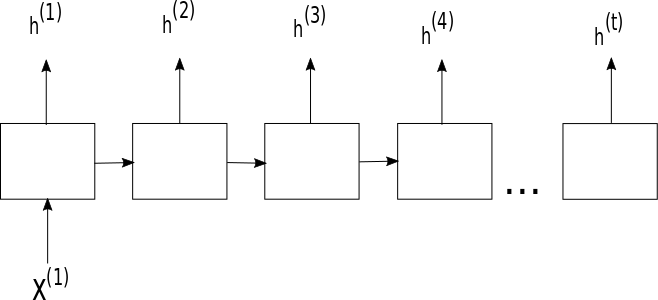
\includegraphics{images/taikymas1.png}}
  \caption{Tinklo apmokymas, kai paduodama viena sakinio raidė.}
  \label{fig:taikymas1}
  \end{figure}
  \item Toliau bus paduodamos dvi pirmos sakinio raidės, kaip įvestis. Pagal šias įvestis bus prognozuojama trečioji sakinio raidė ir tinklas bus apmokomas lyginant šią raidę su duotojo sakinio trečiąja raide. Šį ciklą taip pat kartosime tol kol įvyks vienas iš dviejų variantų paminėtų pirmame punkte.
  \begin{figure}[h!]
    \centering
  \scalebox{0.6}{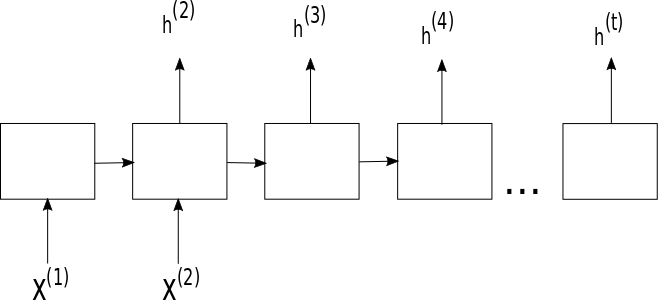
\includegraphics{images/taikymas2.png}}
  \caption{Tinklo apmokymas, kai paduodamos dvi sakinio raidės.}
  \label{fig:taikymas2}
  \end{figure}
  \item Tokiu būdu didinsime paduodamų sakinio raidžių kiekį, kaip įvestis. Pagal šias įvestis prognozuosime sekančią sakinio raidę, kurią lyginant su atitinkama duotojo sakinio raide apmokinsime tinklą. Šį ciklą kartosime iki tol kol įvyks vienas iš dviejų variantų paminėtu prieš tai buvusiuose punktuose arba paduodamų sakinio raidžių kiekis sutaps su duotuoju sakiniu.
  \begin{figure}[h!]
    \centering
  \scalebox{0.6}{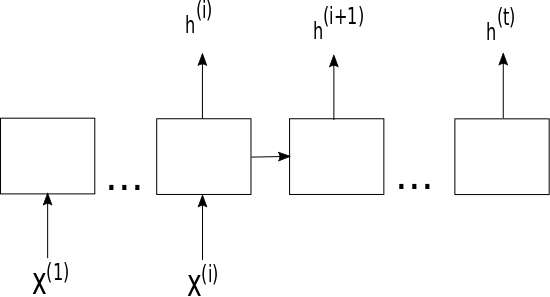
\includegraphics{images/taikymas4.png}}
  \caption{Tinklo apmokymas, kai paduodamos kelios sakinio raidės.}
  \label{fig:taikymas3}
  \end{figure}
\end{enumerate}


\subsection{Programinė įranga}
Darbe kurtas rekurentinis neuroninis tinklas buvo realizuotas C++ programavimo kalba. Naudojama operacinė sistema yra Ubuntu, kuri yra sukurta Linux pagrindu. Projektas buvo saugomas gitHub repozitorijoje.
\clearpage

\begin{figure}[h!]
  \centering
\scalebox{0.45}{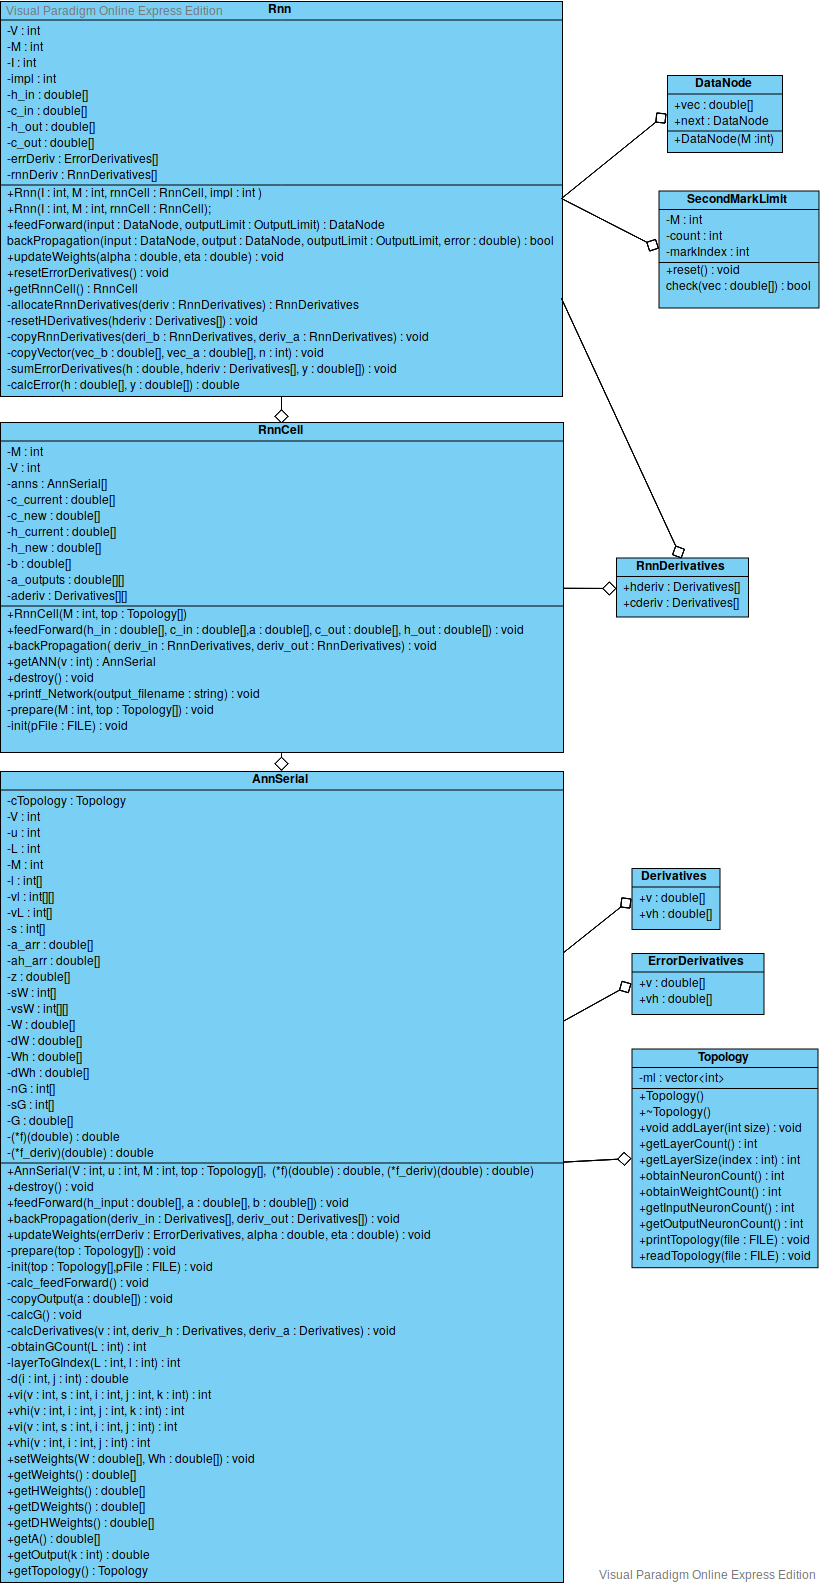
\includegraphics[trim=0 0 0 0cm, clip]{images/new_diag2.png}}
\caption{Klasiu diagrama}
\label{fig:classdiag}
\end{figure}

\clearpage
Tinklui realizuoti buvo sukurtos klasės, kurios aprašo tinklo veikimą.

\begin{enumerate}
  \item \textbf{Rnn} - klasė, kuri kontroliuoja viso tinklo veikimą. Apdoroja įvesties duomenis, apskaičiuoja prognozuojamas reikšmes, tinklą apmokina.
  \item \textbf{RnnCell} - klasė, kuri kontroliuoja rekurentinio neuroninio tinklo skaičiavimus susijusius su viena apmokymo ar prognozavimo iteracija.
  \item \textbf{AnnSerial} - klasė, kuri kontroliuoja paprastų neuroninų tinklų skaičiavimus susijusius su viena apmokymo ar prognozavimo iteracija.
  \item \textbf{Topology} - klasė, kuri saugo atitinkamo neuroninio tinklo struktūrą.
  \item \textbf{Derivatives} - klasė. kuri saugo atitinkamo tinklo išvesčių išvestines, pagal atitinkamo neuroninio tinklo svorius.
  \item \textbf{ErrorDerivatives} - klasė. kuri saugo viso tinklo išvesčių išvestines, pagal atitinkamo neuroninio tinklo svorius.
  \item \textbf{RnnDerivatives} - klasė, kuri saugo visų tinklų išvestines, pagal visų tinklų svorius.
  \item \textbf{SecondMarkLimit} - klasė, kuri skaičiuoja kiek kartų atitinkamas simbolis buvo panaudotas, pagal kurį yra prognozuojamas tekstas.
\end{enumerate}

\clearpage

\begin{figure}[h!]
  \centering
\scalebox{0.8}{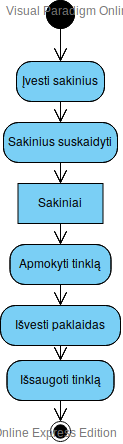
\includegraphics[trim=0 0 0 0cm, clip]{images/Drawing0.png}}
\caption{Veiklos diagrama.}
\label{fig:activity}
\end{figure}

\ref{fig:activity} paveiksle pavaizduota tinklo apmokymo veiklos diagrama. Iš pradžių yra paduodami duomenys į tinklą, šie duomenys yra suskaidomi į sąkinius. Tinklas apmokomas tinklą apmokinant kas vieną sakinį ir grąžinant to sakinio apmokymo vidutinės paklaidos reikymę. Kai yra apmokomi visi sakiniai tinklas gražina kiek laiko mokinosi ir išsisaugo apmokinto tinklo parametrus, kad jį būtų galima naudoti ateityje prognozuojant reikšmes.


% \clearpage

% \section{LSTM taikymo idėja}
% Kur ir kaip taikome LSTM


\clearpage

\section{Eksperimentiniai skaičiavimai}
Šioje dalyje apmokant tinklą analizuosiu tinklo apmokymą apibūdinančius parametrus:
\begin{enumerate}
  \item Palyginsiu tinklo apmokymo vidutines paklaidas, kai tinklo naujam apmokymui yra naudojamos praeito apmokymo dalinės išvestinės su tinklo apmokymu, kai dalinės išvestinės po kiekvienos apmokymo iteracijos yra nunulinamos.
  \item Lyginsiu tinklo vidutines paklaidas priklausant nuo apmokymų skačiaus su skirtingomis $\alpha$ ir $\eta$ reikšmėms.
  \item Lyginsiu tinklo apmokymo vidutines paklaidas didėjant apmokymo duomenų kiekiui.
  \item Atliksiu tinklo apmokymo greitaveikos tyrimą, esant skirtingoms tinklo topologijoms.
  % \item Palyginsiu tinklo apmokymo greitį skaičiavimus atliekant ant CPU ir GPU.
\end{enumerate}

\begin{enumerate}
  \item\textbf{Tinklo apmokymo vidutinių paklaidų lyginimas, kai naujam tinklo apmokymui yra naudojamos praeito žingsnio dalinės išvestinės su tinklo apmokymu, kai dalinės išvestinės po kiekvieno apmokymo yra nunulinamos.}

Šis tyrimas bus atliekamas, kai prie vienodų tinklo parametrų.
$\alpha = 0.8$
$\eta = 0.2$
Topologija - įvesties h reikšmių bus M, įvesties x reikšmių bus I+1, išvesties reikšmių, taip pat bus M.

Abiejais atvejais bus vykdomas apmokymas atliekant n=100 epochų.

Lyginsime tinklo vidutines paklaidas po kiekvienos apmokymo epochos. (\ref{fig:paklaidos1})

\begin{figure}[h!]
  \centering
\scalebox{0.6}{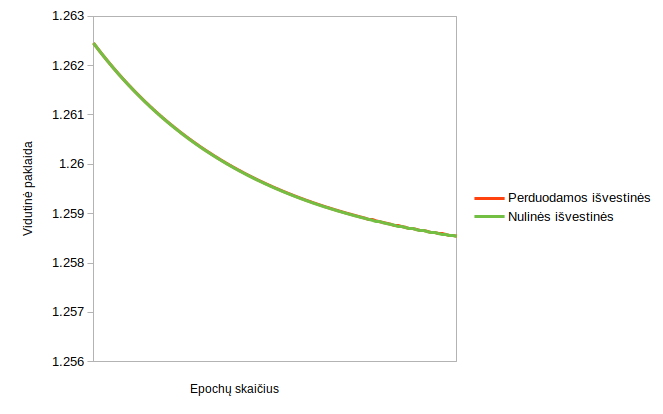
\includegraphics{images/paklaida.png}}
\caption{Apmokymo paklaidos.}
\label{fig:paklaidos1}
\end{figure}

Tinklą apmokant naudojant abu būdus, tinklo apmokymo klaidos funkcijų grafikai yra identiški, todėl nėra būtina šių paklaidų perduoti atliekant naują apmokymą.

\item \textbf{Lyginsiu tinklo vidutines paklaidas priklausant nuo apmokymų skačiaus su skirtingomis $\alpha$ ir $\eta$ reikšmėms.}


\item \textbf{Lyginsiu tinklo apmokymo vidutines paklaidas didėjant apmokymo duomenų kiekiui.}


\item \textbf{Atliksiu tinklo apmokymo greitaveikos tyrimą, esant skirtingoms tinklo topologijoms.}




\end{enumerate}


\clearpage

\section{Išvados}
\begin{enumerate}
  \item Buvo sudarytos ir išvestos LSTM rekurentinio neuroninio tinklo formulės. Pavyko išvesti bendrąsias tinklo apmokymo formules gradientinio nusileidimo metodu. Šios formulės buvo optimizuotos, naudojant algoritmų analizės dinaminio programavimo metodą, kai tinklo išvesčių reikšmių išvestinės apskaičiuojamos nenaudojant rekurencijos "top-down" metodika, o naudojama "bottom-up" metodika, kai iš pradžių yra apskaičiuojamos tarpinės reikšmės, jos išsaugomos ir apjungiamos.
  \item Tinklas buvo realizuotas programiškai. Tinklas implementuotas taip, kad būtų galima patogiai keisti įvesties ir išvesties vektorių ilgius, būtų galima pasirinkti kiekvieno viduje esančio neuroninio tinklo individualias topologijas, nustatyti šių tinklų naudojamas aktyvacijos funkcijas ir pasirinkti apmokymui naudojamų parametrų reikšmes.
  \item Tinklo atskiri metodai buvo ištestuoti ir metodai veikia korektiškai.
  \item Tinklas yra pritaikytas apmokymui duotuoju tekstu ir tada tinklas išsaugomas faile. Šį tinklą poto galima pasileisti ir prognozuoti sakinius, tačiau tinklui korektiškai prognozuoti tekstą reikia atlikti labai daug apmokymų.
  \item
  \begin{enumerate}
    \item Apmokant tinklą nėra būtina perduoti naujai apskaičiuotų išvestinių į tolimesnių žingsnių apmokymus, kadangi tinklas yra apmokomas vienodai abiejais atvejais. Remiantis šiuo faktu galima supaprastinti išvestas formules, kurias realizavus tinklo apmokymo laikas būtų daug trumpesnis.
    \item Naudojant skirtingus apmokymo parametrus tinklas apsimokina skirtingai, tačiau visus atvejus sieja, kad apmokant šį tinklą naudojant bet kokius parametrus, tinklo funkcija patenka į lokalaus minimumo tašką, dėl kurio tinklas pilnai neapsimoko.
    \item Tinklo apmokymas, kai įvesties reikšmių vektorių ir prognozuojamų reikšmių vektorių ilgiai didėja, tai tinklo apmokymo trukmė didėja eksponentiškai, todėl apmokant tinklą įvesties reikšmių parametrus būtų galima klasifikuoti į klases, kurios leistų tinklui greičiau apsimokinti.
  \end{enumerate}
\end{enumerate}


\clearpage

\section*{Literatūros sąrašas}
\addcontentsline{toc}{section}{Literatūros sąrašas}

\begingroup
   \renewcommand{\section}[2]{}%
   \bibliographystyle{iso}
   \bibliography{db}
\endgroup

\clearpage
\section{Priedai}
\subsection{ann.h failas}

//
// Random
//
class Random {
  private:
    std::mt19937 *mGen;
    std::uniform\_real\_distribution<double> *mDist;

  public:
    Random();
    double next();
    int nextInt(int min, int max);
    bool nextBool();
};


class Topology {
	private:
		std::vector<int> *ml;
	public:
		Topology();
		~Topology();

		void addLayer(int size);

		int getLayerCount();
		int getLayerSize(int index);
		int obtainNeuronCount();
		int obtainWeightCount();
		int getInputNeuronCount();
		int getOutputNeuronCount();
    void printTopology(FILE *file);
    void readTopology(FILE *file);
};

struct Derivatives{
  double *v;
  double *vh;
};

template <typename T>
class AnnBase {
  public:
    virtual void feedForward(T *h\_input, T *a, T *b) = 0; // MB: h, a->x, b->a
    virtual void backPropagation(Derivatives **deriv\_in, Derivatives **deriv\_out);
    virtual void destroy() = 0;

  private:
    virtual void prepare(Topology **top, int M)=0; // MB: M
    virtual	void init(FILE *pFile)=0; // MB: pFile neraikia kol kas
    virtual void reset()=0;
    virtual void calc\_feedForward()=0;
    virtual void copyOutput(double *a)=0;
};



class AnnSerial{ // -> AnnSerial
private:
  Topology* cTopology;
  int V; // total number of ANNs
  int u; // index of ANN
  int L;
  int M;
  int * l; // neuronu skaičius sluoksnyje
  int **vl;
  int *vL;
  int * s; // sluoksnio pradzios indeksai
  double * a\_arr;
  double * ah\_arr;
  double * z;
  int * sW;
  int ** vsW;

  double * W;
  double * dW;
  double * Wh;
  double * dWh;


  int * nG;
  int * sG;//pazieti kurie int kurie double
  double * G;

  double (*f)(double);
  double (*f\_deriv)(double);


public:

  AnnSerial(int V, int u, int M, Topology **top,  double (*f)(double), double (*f\_deriv)(double));

  void destroy();

  void feedForward(double *h\_input, double *a, double *b); // ...
  void backPropagation(Derivatives **deriv\_in, Derivatives **deriv\_out);

  void updateWeights(ErrorDerivatives *errDeriv, double alpha, double eta);

private:

  void prepare(Topology **top);
  void init(Topology **top,FILE *pFile);

  void calc\_feedForward();
  void copyOutput(double *a);

  void calcG();
  void calcDerivatives(int v, Derivatives *deriv\_h, Derivatives *deriv\_a);
  int obtainGCount(int L);
  int layerToGIndex(int L, int l);
  double d(int i, int j);

public:
  int vi(int v, int s, int i, int j, int k);
  int vhi(int v, int i, int j, int k);

  int vi(int v, int s, int i, int j);
  int vhi(int v, int i, int j);


  void setWeights(double *W, double *Wh);

  double* getWeights();
  double* getHWeights();
  double* getDWeights();
  double* getDHWeights();
  double* getA();
  double getOutput(int k);

  Topology* getTopology();
};

//
// Global functions
//

void obtainSW(Topology *top, int *sW);


\subsection{ann.cpp failas}


//
// Random
//
Random::Random(){
  mGen = new std::mt19937();
  mDist = new std::uniform\_real\_distribution<double>(0., 1.);
}

double Random::next(){
  return (*mDist)(*mGen);
}

int Random::nextInt(int min, int max){
  double range = max - min;
  double r = range * next();
  return min + (int)(r+0.5);
}

bool Random::nextBool(){
  if(next() >= 0) return true;
  return false;
}

//*****************************
//
// Topology
//
Topology::Topology(){
	ml = new vector<int>();
}

Topology::~Topology(){
	ml->clear();
	delete ml;
}

void Topology::addLayer(int size){
	ml->push\_back(size);
}

int Topology::getLayerCount(){
	return ml->size();
}

int Topology::getLayerSize(int index){
	return (*ml)[index];
}

int Topology::obtainNeuronCount(){
	int count = 0;
	for (int i = 0; i < ml->size(); i++)
		count += (*ml)[i] + 1;
  count--;
	return count;
}

int Topology::obtainWeightCount(){
	int count = 0;
	for (int i = 0; i < ml->size()-1; i++)
		count += ((*ml)[i] + 1)*(*ml)[i+1];
	return count;
}

int Topology::getInputNeuronCount(){
	return (*ml)[0];
}

int Topology::getOutputNeuronCount(){
	return (*ml)[ml->size()-1];
}

void Topology::printTopology(FILE *file){
  int a=getLayerCount();
  fwrite (\&a , sizeof(int), 1, file);
  for(int i=0;i<a;i++){
    int b=ml->at(i);
    fwrite (\&b , sizeof(int), 1, file);
  }
}

void Topology::readTopology(FILE *file){
  int size=0;
  (void)fread (\&size , sizeof(int), 1, file);
  int* abc=new int[size];
  ml=new vector<int>();
  (void)fread (abc , sizeof(int), size, file);
  for(int i=0;i<size;i++){
    ml->push\_back(abc[i]);
  }
}



//***********************************
//
// AnnSerial
//

AnnSerial::AnnSerial(int V, int u, int M, Topology **top, double (*f)(double), double (*f\_deriv)(double)){
  this->V = V;
  this->u = u;
  this->M = M;
  cTopology = new Topology();
    cTopology = top[u];

  L = cTopology->getLayerCount();

  this->f=(*f);
  this->f\_deriv=(*f\_deriv);

  assert(M == top[u]->getOutputNeuronCount());
  prepare(top);

  init(top, NULL);
}

void AnnSerial::destroy(){
	delete[] l;
	l = NULL;

  delete [] vl;
  vl = NULL;

  delete[] vL;
  vL= NULL;

	delete[] s;
	s = NULL;

	delete[] a\_arr;
	a\_arr = NULL;

  delete[] ah\_arr;
  ah\_arr = NULL;

	delete[] z;
	z = NULL;

	delete[] sW;
	sW = NULL;

  delete [] vsW;
  vsW = NULL;

	delete[] W;
	W = NULL;
	delete[] dW;
	dW = NULL;

  delete[] Wh;
  Wh = NULL;
  delete[] dWh;
  dWh = NULL;

  delete[] nG;
  nG = NULL;
  delete[] sG;
  sG = NULL;


	// delete[] t\_arr;
	// t\_arr = NULL;

	// delete[] gjl;
	// gjl = NULL;
}

void AnnSerial::prepare(Topology **top){

  vL = new int[V];
  vl = new int*[V];
  for(int i = 0; i < V; i++){
    vl[i] = new int[top[u]->getLayerCount()];
  }
	l = new int[cTopology->getLayerCount()];
	s = new int[cTopology->getLayerCount()];

	int neuronCount = cTopology->obtainNeuronCount();
	int weightCount = cTopology->obtainWeightCount();

	a\_arr = new double[neuronCount];
	z = new double[neuronCount];

  ah\_arr = new double[M];

  vsW = new int*[V];
  for(int v = 0; v < V; v++)
    vsW[v] = new int[top[v]->getLayerCount()-1];

	sW = new int[cTopology->getLayerCount()-1];

	W = new double[weightCount];
	dW = new double[weightCount];

  int second\_layer\_size = cTopology->getLayerSize(1);
  int h\_weightCount = second\_layer\_size * M;

  Wh = new double[h\_weightCount];
  dWh = new double[h\_weightCount];

  int G\_count = obtainGCount(L);


  nG = new int[G\_count];
  sG = new int[G\_count];

  int count = 0;
  int l2;
  for(int gl = 0; gl < G\_count; gl++){
    l2 = L - 2*gl - 1;
    nG[gl] = cTopology->getLayerSize(l2)*(cTopology->getLayerSize(l2 - 2));
    count += nG[gl];
  }


  for(int gl = 0; gl < G\_count; gl++){
    if(gl == 0)
      sG[0] = 0;
    else
      sG[gl] = sG[gl-1] + nG[gl-1];
  }

  G = new double[count];


	//gjl = new double[neuronCount];
}

void AnnSerial::init(Topology **top,FILE * pFile=NULL){

	Random *rnd = new Random();

	//Neuronu kiekiai sluoksnyje
	for (int i = 0; i < L; i++) {
		l[i] = cTopology->getLayerSize(i) + 1;
	}

	//Sluoksniu pradzios indeksai
	for (int i = 0; i < L; i++) {
		s[i] = 0;
		for (int j = i; j > 0; j--) {
			s[i] += l[j - 1];
		}
	}

	//Bias neuronai
	for (int i = 0; i < L - 1; i++) {
		a\_arr[s[i + 1] - 1] = 1;
	}

  for(int i = 0; i < V; i++){
    vL[i] = top[i]->getLayerCount();
  }

  for(int i = 0; i < V; i++)
    for(int j = 0; j < vL[i]; j++)
      vl[i][j] = top[i]->getLayerSize(j)+1;


	//Svoriu kiekiai l-ame sluoksnyje


  obtainSW(top[u], sW);
  for(int v = 0; v < V; v++){
    obtainSW(top[v], vsW[v]);
  }


  if (pFile==NULL) {
    for (int ll = 0; ll < L - 1; ll++)
      for (int i = 0; i < l[ll]; i++)
        for (int j = 0; j < l[ll+1]-1; j++){
          W[sW[ll] + i*(l[ll+1]-1) + j] = (rnd->next()*2-1);
          dW[sW[ll] + i*(l[ll+1]-1) + j] = 0.0;
        }


    int second\_layer\_size = cTopology->getLayerSize(1);
    int h\_weightCount = second\_layer\_size * M;
    for(int i = 0; i < M; i++)
      for(int j = 0; j < l[1]-1; j++)
        Wh[i*(l[1]-1) + j] = (rnd->next()*2-1);

  }
  else {
  //  readf\_Network(pFile);
  }

  delete rnd;

}

void AnnSerial::updateWeights(ErrorDerivatives *errDeriv, double alpha, double eta){

  for(int k = 0; k < cTopology->obtainWeightCount(); k++){
    dW[k] = -eta*errDeriv->v[k] + alpha*dW[k];
    W[k] = W[k] + dW[k];
  }

  for(int k = 0; k < cTopology->getLayerSize(1)*M; k++){
    dWh[k] = -eta*errDeriv->vh[k] + alpha*dWh[k];
    Wh[k] = Wh[k] + dWh[k];
  }

}

void AnnSerial::feedForward(double *h\_input, double *a, double *b){

  for (int i = 0; i < cTopology->getLayerSize(0); i++) {
    a\_arr[i] = a[i];
  }
  a\_arr[cTopology->getLayerSize(0)] = 1.0;

  for(int i=0; i<M;i++){
    ah\_arr[i] = h\_input[i];
  }

	calc\_feedForward();

	copyOutput(b);
}

void AnnSerial::calc\_feedForward(){

  for (int j = 0; j < cTopology->obtainNeuronCount(); j++) {
		z[j] = 0;
	}
  for(int k = 0; k < l[1] - 1; k++){
    for(int j = 0; j < M; j++){
      z[s[1] + k] += ah\_arr[j] * Wh[j*(l[1]-1) + k];
    }
  }
	for (int i = 0; i < L - 1; i++) {//per sluoksnius einu+
    for (int k = 0; k < l[i + 1] - 1; k++) {//per sekancio sluoksnio z+
		  for (int j = 0; j < l[i]; j++) { //kiek neuronu sluoksnyje+
				z[s[i + 1] + k] += W[sW[i] + j*(l[i + 1] - 1) + k] * a\_arr[s[i] + j];
			}
		}
		for (int k = 0; k < l[i + 1] - 1; k++) {//per sekancio sluoksnio z
			a\_arr[s[i + 1] + k] = f(z[s[i + 1] + k]);
		}
	}
}

void AnnSerial::copyOutput(double *a){
  for (int i = 0; i<cTopology->getLayerSize(cTopology->getLayerCount() - 1); i++)
		a[i] = a\_arr[s[L - 1] + i];
}

void AnnSerial::backPropagation(Derivatives **deriv\_in, Derivatives **deriv\_out){

  calcG();

  for(int v = 0; v < V; v++)
    calcDerivatives(v, deriv\_in[v],  deriv\_out[v]);
}

void AnnSerial::calcG(){
  int G\_count = obtainGCount(L);
  int l2;
  for(int gl = 0; gl < G\_count; gl++){
    l2 = L - 2*gl - 1;

    double sum = 0;

    if(l2==2){

      for(int p = 0; p < M; p++){
        for(int k = 0; k < l[l2]-1; k++){

          for(int n = 0; n < l[l2-1]-1; n++){
            sum += Wh[(l[l2-1]-1)*p + n]*W[sW[l2-1] + (l[l2]-1)*n + k]*f\_deriv(z[s[l2-1]+n]);
            //pakeiciau W i Wh
            //sum += Wh[M*p + n]*W[sW[l2-1] + (l[l2]-1)*n + k]*f\_deriv(z[s[l2-1]+n]);
          }

          G[sG[gl] + (l[l2]-1)*p + k] = f\_deriv(z[s[l2] + k])*sum;
        }

      //  G[sG[gl] + (l[l2]-1)*p + k] = f\_deriv(z[s[l2] + k])*sum;
      }

    }else{
      for(int p = 0; p < l[l2-2]; p++){
        for(int k = 0; k < l[l2]-1; k++){

          for(int n = 0; n < l[l2-1]-1; n++){
            sum += W[sW[l2-2] + (l[l2-1]-1)*p + n]*W[sW[l2-1] + (l[l2]-1)*n + k]*f\_deriv(z[s[l2-1]+n]);
          }

          G[sG[gl] + (l[l2]-1)*p + k] = f\_deriv(z[s[l2] + k])*sum;
        }
      }
    }
  }
}

void AnnSerial::calcDerivatives(int v, Derivatives *deriv\_in, Derivatives *deriv\_out){
  // deriv\_in->v[vi(...)];
  // deriv\_in->vh[vhi(...)];

  int max\_layer\_size = 0;
  for(int i = 0; i < L; i++)
    max\_layer\_size = (l[i]-1) > max\_layer\_size ? l[i]-1 : max\_layer\_size;

  // vec0 -> vec1
  double *vec0 = new double[max\_layer\_size];
  double *vec1 = new double[max\_layer\_size];


  int start\_l = L%2 == 1 ? 0 : 1;

    for(int ss = 0; ss < vL[v]-1; ss++){//kiek sluoksniu tinkle
      for(int wi = 0; wi < vl[v][ss]; wi++){//kiek neuronu
        for(int wj = 0; wj < vl[v][ss+1]-1; wj++){//kiek sekanciame neuronu
          for(int ll = start\_l; ll < L; ll=ll+2){//per G reiksmes  cia gal maziau tik

            if(ll == 0){

              for(int k = 0; k < M; k++)
                vec1[k] = deriv\_in->v[vi(v, ss, wi, wj, k)];

            }else if(ll == 1){

              for(int k = 0; k < l[ll]-1;k++){
                double sum = 0;
                for(int n = 0; n < M; n++){
                  sum += Wh[(l[ll]-1)*n + k]*deriv\_in->v[vi(v, ss, wi, wj, n)];
                }

                if(u == v) sum += a\_arr[wi];

                vec1[k] = f\_deriv(z[s[ll] + k])*sum;
              }


            }else {


              int gl = layerToGIndex(L, ll);
              double sum = 0;
              int to\_p = ll == 2 ? M : l[ll-2]-1;//-1 gal


              for(int k = 0; k < l[ll]-1;k++){
                for(int p = 0; p < to\_p; p++){
                  sum += vec0[p]*G[sG[gl] + (l[ll]-1)*p + k];
                }


                if(u == v){
                  if(ll == ss+1)
                    sum += f\_deriv(z[s[ll] + k])*a\_arr[s[ll-1] + wi];
                  else if(ll == ss+2){
                      double sum2 = 0;
                      for(int n = 0; n < l[ll-1]; n++)
                       sum2 += W[sW[ll-1] + (l[ll]-1)*n + k] * f\_deriv(z[s[ll-1] + n]);
                      sum += f\_deriv(z[s[ll] + k])*a\_arr[s[ll-2] + wi]*sum2;
                  }
                }
              }
            }
            int to\_k = ll == 0 ? M : l[ll]-1;
            for(int k = 0; k < to\_k; k++) vec0[k] = vec1[k];

          }
          for(int k = 0; k < M /*l[L-1]-1*/; k++){
            deriv\_out->v[vi(v, ss, wi, wj, k)] = vec1[k];

          }
        }
      }
    }

      for(int wi = 0; wi < M; wi++){//kiek neuronu
        for(int wj = 0; wj < vl[v][1]-1; wj++){//kiek sekanciame neuronu
          for(int ll = start\_l; ll < L; ll=ll+2){//per G reiksmes  cia gal maziau tik
            if(ll == 0){

              for(int k = 0; k < M; k++)
                vec1[k] = deriv\_in->vh[vhi(v, wi, wj, k)];

            }else if(ll == 1){

              for(int k = 0; k < l[ll]-1;k++){
                double sum = 0;
                for(int n = 0; n < M; n++)
                  sum += Wh[(l[ll]-1)*n + k]*deriv\_in->vh[vhi(v, wi, wj, n)];
                if(u == v ) sum += ah\_arr[wi];
                vec1[k] = f\_deriv(z[s[ll] + k])*sum;

              }

            }else {


              int gl = layerToGIndex(L, ll);
              double sum = 0;
              int to\_p = ll == 2 ? M : l[ll-2]-1;//-1 gal


              for(int k = 0; k < l[ll]-1;k++){
                for(int p = 0; p < to\_p; p++){
                  sum += vec0[p]*G[sG[gl] + (l[ll]-1)*p + k];
                }


                if(u == v){

                  if(ll == 2){
                    double sum2 = 0;
                    for(int n = 0; n < l[ll-1]; n++)
                      sum2 += W[sW[ll-1] + (l[ll]-1)*n + k] * f\_deriv(z[s[ll-1] + n]);
                    sum += f\_deriv(z[s[ll] + k])*ah\_arr[wi]*sum2;
                  }
                }
              }
            }

            int to\_k = ll == 0 ? M : l[ll]-1;
            for(int k = 0; k < to\_k; k++) vec0[k] = vec1[k];
          }

          for(int k = 0; k < M /*l[L-1]-1*/; k++){
            deriv\_out->vh[vhi(v, wi, wj, k)] = vec1[k];
          }
        }
      }

  delete [] vec0;
  delete [] vec1;

}

int AnnSerial::obtainGCount(int L){
  int G\_count = 0;
  int remaining\_L = L;
  while(remaining\_L >= 3){
    G\_count++;
    remaining\_L -= 2;
  }
  return G\_count;
}

int AnnSerial::layerToGIndex(int L, int l){
  int G\_count = obtainGCount(L);
  return G\_count - (l - l%2) / 2;
}

int AnnSerial::vi(int v, int s, int i, int j, int k){
  return (vsW[v][s] + i*(vl[v][s+1]-1) + j)*M + k;
}

int AnnSerial::vhi(int v, int i, int j, int k){
  return  (i*(vl[v][1]-1) + j)*M + k;
}

int AnnSerial::vi(int v, int s, int i, int j){
  return vsW[v][s] + i*(vl[v][s+1]-1) + j;
}

int AnnSerial::vhi(int v, int i, int j){
  return  i*(vl[v][1]-1) + j;
}

double AnnSerial::d(int i, int j){
  if(i == j) return 1.0;
  return 0.0;
}

void AnnSerial::setWeights(double *W, double *Wh){
  this->W = W;
  this->Wh = Wh;
};

double* AnnSerial::getWeights(){
	return W;
}

double* AnnSerial::getDWeights(){
	return dW;
}

double* AnnSerial::getHWeights(){
	return Wh;
}

double* AnnSerial::getDHWeights(){
	return dWh;
}

double* AnnSerial::getA(){
	return a\_arr;
}

double AnnSerial::getOutput(int k){
  return a\_arr[s[L-1]+k];
}


Topology* AnnSerial::getTopology(){
  return cTopology;
}

//
// Global functions
//


void obtainSW(Topology *top, int *sW){
  int nW;
  sW[0] = 0;
  for (int i = 1; i < top->getLayerCount()-1; i++) {
		nW = (top->getLayerSize(i-1)+1)*top->getLayerSize(i); //l[i] * (l[i + 1] - 1);
    sW[i] = sW[i-1] + nW;
  }
}

\subsection{rnn.h failas}

class Topology;
class AnnSerial;
struct Derivatives;

/* Class definitions here. */
void run\_cuda\_sample();

class RnnConfig{
private:
  Topology** cTopology;
  int mM;


public:
  void setTopologies(Topology **top);
  void setM(int M);


  Topology** getTopologies();
  int getM();

};



struct RnnDerivatives {
  Derivatives **hderiv;
  //+hderiv : Derivatives[]
  Derivatives **cderiv;
  //+cderiv : Derivatives[]
};

struct ErrorDerivatives {
  double *v;
  //+v : double[]
  double *vh;
  //+vh : double[]
};

template <typename T>
class RnnBase {
  public:
  	 virtual void train(T *a, T *b, T alpha, T eta) = 0;
  	 virtual void feedForward(T *h\_in, T *c\_in,T *a, T *c\_out, T *h\_out) = 0;


  private:
     virtual	void init(FILE *pFile)=0;
};


class RnnCell {
  private:

    int M;
    //-M : int
    int V;
    //-V : int

    AnnSerial** anns;
    //-anns : AnnSerial[]
    AnnSerial* ann\_forget; // 0

    AnnSerial* ann\_input; // 1
    AnnSerial* ann\_gate; // 2
    AnnSerial* ann\_output; // 3

    double* c\_current;
    //-c\_current : double[]
    double* c\_new;
    //-c\_new : double[]
    double* h\_current;
    //-h\_current : double[]
    double* h\_new;
    //-h\_new : double[]
    double* b;
    //-b : double[]
    double** a\_outputs;
    //-a\_outputs : double[][]

    Derivatives ***aderiv;
    //-aderiv : Derivatives[][]




  public:

    RnnCell(int M, Topology **top) {
      prepare(M, top);
      init(NULL);
    };
    //+RnnCell(M : int, top : Topology[])


    RnnCell(int M, string filename);



  	 void feedForward(double *h\_in, double *c\_in,double *a, double *c\_out, double *h\_out);
     //+feedForward(h\_in : double[], c\_in : double[],a : double[], c\_out : double[], h\_out : double[]) : void
     void backPropagation( RnnDerivatives *deriv\_in, RnnDerivatives *deriv\_out);
     //+backPropagation( deriv\_in : RnnDerivatives, deriv\_out : RnnDerivatives) : void

    //
    AnnSerial* getANN(int v);
    //+getANN(v : int) : AnnSerial

    void destroy();
    //+destroy() : void

    void printf\_Network(string output\_filename);

    //+printf\_Network(output\_filename : string) : void
  private:
    void prepare(int M, Topology **top);
    //-prepare(M : int, top : Topology[]) : void
    void init(FILE *pFile);
    //-init(pFile : FILE) : void

};


class OutputLimit {
  public:
    virtual void reset() = 0;
    virtual bool check(double *vec) = 0;
};

class SecondMarkLimit : public OutputLimit {
  private:
    int M;
    int count;
    int markIndex;

  public:
    SecondMarkLimit(int markIndex, int M);

    void reset();
    bool check(double *vec);
};

struct DataNode{
  DataNode(int M);
  double* vec;
  DataNode *next;
};


class Rnn {
  private:
    int I;
    int M;
    int V;

    RnnCell* cRnnCell;


    double *h\_in;
    double *h\_out;
    double* c\_in;
    double *c\_out;

    ErrorDerivatives** errDeriv;
    RnnDerivatives **rnnDeriv;

    int impl;

  public:
    Rnn(int I, int M, RnnCell *rnnCell, int impl);
    Rnn(int I, int M, RnnCell *rnnCell);

    DataNode* feedForward(DataNode* input, OutputLimit *outputLimit);
    bool backPropagation(DataNode* input, DataNode* output, OutputLimit *outputLimit, double \&error);

    void updateWeights(double alpha, double eta);
    //+updateWeights(alpha : double, eta : double) : void
    void resetErrorDerivatives();
    //+resetErrorDerivatives() : void


    RnnCell* getRnnCell(){
      return cRnnCell;
    }

    //+getRnnCell() : RnnCell

  private:

    RnnDerivatives* allocateRnnDerivatives(RnnDerivatives* deriv);
    //-allocateRnnDerivatives(deriv : RnnDerivatives) : RnnDerivatives

    //RnnDerivatives* deallocateRnnDerivatives(RnnDerivatives* deriv);
    void resetHDerivatives(Derivatives** hderiv);
    //-resetHDerivatives(hderiv : Derivatives[]) : void
    void resetCDerivatives(Derivatives** cderiv);


    void copyRnnDerivatives(RnnDerivatives* deri\_b, RnnDerivatives* deriv\_a);
    //-copyRnnDerivatives(deri\_b : RnnDerivatives, deriv\_a : RnnDerivatives) : void
    void copyVector(double* vec\_b, double *vec\_a, int n);
    //-copyVector(vec\_b : double[], vec\_a : double[], n : int) : void

    void sumErrorDerivatives(double *h, Derivatives **hderiv, double *y);
    //-sumErrorDerivatives(h : double, hderiv : Derivatives[], y : double[]) : void
    double calcError(double *h, double *y);
    //-calcError(h : double[], y : double[]) : double


};

double f(double x);
double f\_deriv(double x);

double f\_tanh(double x);
double f\_tanh\_deriv(double x);



\subsection{rnn.cpp failas}

/* C++ code here. */
void RnnConfig::setTopologies(Topology **top){
  cTopology = top;
}

void RnnConfig::setM(int M){
  mM=M;
}


Topology** RnnConfig::getTopologies(){
  return cTopology;
}

int RnnConfig::getM(){
  return mM;
}


//
// RnnCell
//

RnnCell::RnnCell(int M, string filename) {
  FILE * p1File;
  p1File = fopen(filename.c\_str(), "rb");

  Topology** top= new Topology*[4];
  top[0] = new Topology();
  top[1] = new Topology();
  top[2] = new Topology();
  top[3] = new Topology();
  top[0]->readTopology(p1File);
  top[1]->readTopology(p1File);
  top[2]->readTopology(p1File);
  top[3]->readTopology(p1File);


  prepare(M,top);

  double* Ww0= new double[top[0]->obtainWeightCount()];
  double* Ww1= new double[top[1]->obtainWeightCount()];
  double* Ww2= new double[top[2]->obtainWeightCount()];
  double* Ww3= new double[top[3]->obtainWeightCount()];

  double* Whw0= new double[M*top[0]->getLayerSize(1)];
  double* Whw1= new double[M*top[1]->getLayerSize(1)];
  double* Whw2= new double[M*top[2]->getLayerSize(1)];
  double* Whw3= new double[M*top[3]->getLayerSize(1)];

  (void)fread (Ww0 , sizeof(double), top[0]->obtainWeightCount(), p1File);
  (void)fread (Whw0 , sizeof(double), M*top[0]->getLayerSize(1), p1File);

  (void)fread (Ww1 , sizeof(double), top[1]->obtainWeightCount(), p1File);
  (void)fread (Whw1 , sizeof(double), M*top[1]->getLayerSize(1), p1File);

  (void)fread (Ww2 , sizeof(double), top[2]->obtainWeightCount(), p1File);
  (void)fread (Whw2 , sizeof(double), M*top[2]->getLayerSize(1), p1File);

  (void)fread (Ww3 , sizeof(double), top[3]->obtainWeightCount(), p1File);
  (void)fread (Whw3 , sizeof(double), M*top[3]->getLayerSize(1), p1File);


  anns[0]->setWeights(Ww0,Whw0);

  anns[1]->setWeights(Ww1,Whw1);

  anns[2]->setWeights(Ww2,Whw2);

  anns[3]->setWeights(Ww3,Whw3);



  init(p1File);
  fclose (p1File);
};


void RnnCell::printf\_Network(string output\_filename){

    FILE * pFile;
    const char * c = output\_filename.c\_str();
    pFile = fopen(c, "wb");
    anns[0]->getTopology()->printTopology(pFile);
    anns[1]->getTopology()->printTopology(pFile);
    anns[2]->getTopology()->printTopology(pFile);
    anns[3]->getTopology()->printTopology(pFile);

    fwrite (anns[0]->getWeights() , sizeof(double), anns[0]->getTopology()->obtainWeightCount(), pFile);
    fwrite (anns[0]->getHWeights() , sizeof(double), anns[0]->getTopology()->getLayerSize(1)*M, pFile);

    fwrite (anns[1]->getWeights() , sizeof(double), anns[1]->getTopology()->obtainWeightCount(), pFile);
    fwrite (anns[1]->getHWeights() , sizeof(double), anns[1]->getTopology()->getLayerSize(1)*M, pFile);

    fwrite (anns[2]->getWeights() , sizeof(double), anns[2]->getTopology()->obtainWeightCount(), pFile);
    fwrite (anns[2]->getHWeights() , sizeof(double), anns[2]->getTopology()->getLayerSize(1)*M, pFile);

    fwrite (anns[3]->getWeights() , sizeof(double), anns[3]->getTopology()->obtainWeightCount(), pFile);
    fwrite (anns[3]->getHWeights() , sizeof(double), anns[3]->getTopology()->getLayerSize(1)*M, pFile);

    fclose (pFile);
}

void RnnCell::prepare(int M, Topology **top){
  this->M = M;
  V = 4;

  double (*func)(double);
  double (*func\_deriv)(double);

  double (*func\_tanh)(double);
  double (*func\_tanh\_deriv)(double);

  func=f;
  func\_deriv = f\_deriv;

  func\_tanh=f\_tanh;
  func\_tanh\_deriv = f\_tanh\_deriv;


  anns = new AnnSerial*[V];
  for(int v = 0; v < V; v++){
    if(v==2){
      anns[v] = new AnnSerial(V, v, M, top, func\_tanh, func\_tanh\_deriv);
    } else {
      anns[v] = new AnnSerial(V, v, M, top, func, func\_deriv);
    }
  }

  ann\_forget = anns[0];
  ann\_input = anns[1];
  ann\_gate = anns[2];
  ann\_output = anns[3];




  b = new double[M];
  c\_current = new double[M];
  c\_new = new double[M];
  h\_current = new double[M];
  h\_new = new double[M];

  a\_outputs = new double*[V];
  for(int v = 0; v < V; v++){
    a\_outputs[v] = new double[M];
  }

  aderiv = new Derivatives**[V];
  for(int u = 0; u < V; u++){
    aderiv[u] = new Derivatives*[V];
    for(int v = 0; v < V; v++){
      aderiv[u][v] = new Derivatives;
      aderiv[u][v]->v = new double[top[v]->obtainWeightCount()*M];
      aderiv[u][v]->vh = new double[M*top[v]->getLayerSize(1)*M];
    }
  }
}


void RnnCell::init(FILE * pFile=NULL){

  for(int i=0; i<M; i++){
    c\_current[i] = 0;
    h\_current[i] = 0;
  }
}

void RnnCell::feedForward(double *h\_in, double *c\_in, double *a\_in, double *c\_out, double *h\_out){

  c\_current = c\_in; // c\_t0, c\_t1,
  h\_current = h\_in;

  for(int v = 0; v < V; v++)
    anns[v]->feedForward(h\_in, a\_in, a\_outputs[v]);

  for(int i=0; i < M; i++){
    c\_new[i] = c\_out[i] = c\_in[i] * a\_outputs[0][i] + a\_outputs[1][i] * a\_outputs[2][i];
    b[i] = tanh(c\_out[i])* a\_outputs[3][i];
  }

  double sumB = 0;
  for(int i = 0; i < M; i++)
    sumB += exp(b[i]);

  for(int i = 0; i < M; i++)
    h\_new[i] = h\_out[i] = exp(b[i]) / sumB;

}


void RnnCell::backPropagation(RnnDerivatives *deriv\_in, RnnDerivatives *deriv\_out){



  for(int u = 0; u < V; u++)
    anns[u]->backPropagation(deriv\_in->hderiv, aderiv[u]);



  for(int v = 0; v < V; v++){

    Topology *vtop = anns[v]->getTopology();
    for(int s = 0; s < vtop->getLayerCount()-1; s++){

      for(int wi = 0; wi < vtop->getLayerSize(s)+1; wi++){

        for(int wj = 0; wj < vtop->getLayerSize(s+1); wj++){


          for(int k = 0; k < M; k++){

            double cderiv = deriv\_in->cderiv[v]->v[anns[v]->vi(v, s, wi, wj, k)];
            // printf("cderiv: %.20f\n", cderiv);
            double a\_forget = ann\_forget->getOutput(k);
            // printf("a\_forget: %.20f\n", a\_forget);
            double c = c\_current[k];
            // printf("c: %.20f\n", c);
            double a\_forget\_deriv = aderiv[0][v]->v[anns[v]->vi(v, s, wi, wj, k)];
            // printf("a\_forget\_deriv: %.20f\n", a\_forget\_deriv);
            double a\_input\_deriv = aderiv[1][v]->v[anns[v]->vi(v, s, wi, wj, k)];
            // printf("a\_input\_deriv: %.20f\n", a\_input\_deriv);
            double a\_gate = ann\_gate->getOutput(k);
            // printf("a\_gate: %.20f\n", a\_gate);
            double a\_input = ann\_input->getOutput(k);
            // printf("a\_input: %.20f\n", a\_input);
            double a\_gate\_deriv = aderiv[2][v]->v[anns[v]->vi(v, s, wi, wj, k)];
            // printf("a\_gate\_deriv: %.20f\n", a\_gate\_deriv);

            deriv\_out->cderiv[v]->v[anns[v]->vi(v, s, wi, wj, k)] = cderiv*a\_forget + c*a\_forget\_deriv + a\_input\_deriv*a\_gate + a\_input*a\_gate\_deriv;
            // printf("cderiv*a\_forget:  %.20f\n", cderiv*a\_forget);
            // printf("c*a\_forget\_deriv:  %.20f\n", c*a\_forget\_deriv);
            // printf("a\_input\_deriv*a\_gate:  %.20f\n", a\_input\_deriv*a\_gate);
            // printf("a\_input*a\_gate\_deriv:  %.20f\n", a\_input*a\_gate\_deriv);
            // printf("cia:  %.20f\n", deriv\_out->cderiv[0]->v[0]);
            // printf("cia:  %.20f\n", deriv\_out->cderiv[0]->v[1]);
            // break;
          }
        }
      }
    }
    // printf("cia:  %.20f\n", deriv\_out->cderiv[0]->v[0]);
    // printf("cia:  %.20f\n", deriv\_out->cderiv[0]->v[1]);


    for(int wi = 0; wi < M /*vtop->getLayerSize(0)*/; wi++){
      for(int wj = 0; wj < vtop->getLayerSize(1); wj++){

        for(int k = 0; k < M; k++){

          double cderiv = deriv\_in->cderiv[v]->vh[anns[v]->vhi(v, wi, wj, k)];
          // if(wi==1 \&\& wj==0\&\& k==0 \&\& v==0) printf("cderiv: %.20f\n", cderiv);

          double a\_forget = ann\_forget->getOutput(k);
          // if(wi==1 \&\& wj==0\&\& k==0\&\& v==0) printf("a\_forget: %.20f\n", a\_forget);

          double c = c\_current[k];
          // if(wi==1 \&\& wj==0\&\& k==0\&\& v==0) printf("c: %.20f\n", c);

          double a\_forget\_deriv = aderiv[0][v]->vh[anns[v]->vhi(v, wi, wj, k)];
          // if(wi==1 \&\& wj==0\&\& k==0\&\& v==0) printf("a\_forget\_deriv: %.20f\n", a\_forget\_deriv);

          double a\_input\_deriv = aderiv[1][v]->vh[anns[v]->vhi(v, wi, wj, k)];
          // if(wi==1 \&\& wj==0\&\& k==0\&\& v==0) printf("a\_input\_deriv: %.20f\n", a\_input\_deriv);

          double a\_gate = ann\_gate->getOutput(k);
          // if(wi==1 \&\& wj==0\&\& k==0\&\& v==0) printf("a\_gate: %.20f\n", a\_gate);

          double a\_input = ann\_input->getOutput(k);
          // if(wi==1 \&\& wj==0\&\& k==0\&\& v==0) printf("a\_input: %.20f\n", a\_input);

          double a\_gate\_deriv = aderiv[2][v]->vh[anns[v]->vhi(v, wi, wj, k)];
          // if(wi==1 \&\& wj==0\&\& k==0\&\& v==0) printf("a\_gate\_deriv: %.20f\n", a\_gate\_deriv);

          deriv\_out->cderiv[v]->vh[anns[v]->vhi(v, wi, wj, k)] = cderiv*a\_forget + c*a\_forget\_deriv + a\_input\_deriv*a\_gate + a\_input*a\_gate\_deriv;
          // if(wi==1 \&\& wj==0 \&\& k==0\&\& v==0) printf("cderiv*a\_forget:  %.20f\n", cderiv*a\_forget);
          // if(wi==1 \&\& wj==0 \&\& k==0\&\& v==0) printf("c*a\_forget\_deriv:  %.20f\n", c*a\_forget\_deriv);
          // if(wi==1 \&\& wj==0 \&\& k==0\&\& v==0) printf("a\_input\_deriv*a\_gate:  %.20f\n", a\_input\_deriv*a\_gate);
          // if(wi==1 \&\& wj==0 \&\& k==0\&\& v==0) printf("a\_input*a\_gate\_deriv:  %.20f\n", a\_input*a\_gate\_deriv);
          // if(wi==1 \&\& wj==0 \&\& k==0\&\& v==0) printf("deriv\_out->cderiv[v]->vh[anns[v]->vhi(v, wi, wj, k)]: %.20f\n", deriv\_out->cderiv[v]->vh[anns[v]->vhi(v, wi, wj, k)]);
        }
      }
    }
  }

  // printf("1%.20f\n", deriv\_out->cderiv[0]->vh[0]);
  // printf("%.20f\n", deriv\_out->cderiv[0]->vh[1]);
  // printf("%.20f\n", deriv\_out->cderiv[0]->vh[2]);
  // printf("4%.20f\n", deriv\_out->cderiv[0]->vh[3]);
  double* sm\_deriv = new double[M*M];


  for(int k = 0; k < M; k++)
    for(int n = 0; n < M; n++)
      if(k == n) sm\_deriv[k*M + n] = h\_new[k]*(1-h\_new[k]);
      else sm\_deriv[k*M + n] = -h\_new[k]*h\_new[n];

      // printf("sm\_deriv[k*M]: %.20f\n", sm\_deriv[0*M]);
      // printf("sm\_deriv[k*M]: %.20f\n", sm\_deriv[1]);

      for(int v = 0; v < V; v++){
        Topology *vtop = anns[v]->getTopology();
        for(int s = 0; s < vtop->getLayerCount()-1; s++){
          for(int wi = 0; wi < vtop->getLayerSize(s)+1; wi++){
            for(int wj = 0; wj < vtop->getLayerSize(s+1); wj++){
              for(int k = 0; k < M; k++){
                double sum = 0;
                for(int n = 0; n < M; n++){
                  double sum2=0;
                  //sm\_deriv[k*M + n]
                  double a\_output\_deriv = aderiv[3][v]->v[anns[v]->vi(v, s, wi, wj, n)];
                  // printf("a\_output\_deriv: %.20f\n", a\_output\_deriv);
                  double a\_output = ann\_output->getOutput(n);
                  // printf("a\_output: %.20f\n", a\_output);
                  double c\_deriv = deriv\_out->cderiv[v]->v[anns[v]->vi(v, s, wi, wj, n)];
                  // printf("c\_deriv: %.20f\n", c\_deriv);
                  sum2 += a\_output\_deriv*f\_tanh(c\_new[n]) + a\_output*f\_tanh\_deriv(c\_new[n])*c\_deriv;
                  // printf("a\_output\_deriv*f\_tanh(c\_new[n]): %.20f\n", a\_output\_deriv*f\_tanh(c\_new[n]));
                  // printf("a\_output*f\_tanh\_deriv(c\_new[n])*c\_deriv: %.20f\n", a\_output*f\_tanh\_deriv(c\_new[n])*c\_deriv);
                  sum2 *= sm\_deriv[k*M+n];

                  sum+=sum2;

                  // printf("sum: %.20f\n", sum);
                }
                deriv\_out->hderiv[v]->v[anns[v]->vi(v, s, wi, wj, k)] = sum;

              }
            }
          }
        }


        for(int wi = 0; wi < M /*vtop->getLayerSize(0)*/; wi++){
          for(int wj = 0; wj < vtop->getLayerSize(1); wj++){
            for(int k = 0; k < M; k++){
              double sum = 0;
              for(int n = 0; n < M; n++){
                //sm\_deriv[k*M + n]
                double a\_output\_deriv = aderiv[3][v]->vh[anns[v]->vhi(v, wi, wj, n)];
                // printf("a\_output\_deriv:%.20f\n", a\_output\_deriv);

                double a\_output = ann\_output->getOutput(n);
                // printf("a\_output:%.20f\n", a\_output);
                double c\_deriv = deriv\_out->cderiv[v]->vh[anns[v]->vhi(v, wi, wj, n)];
                // printf("c\_deriv:%.20f\n", c\_deriv);
                sum += a\_output\_deriv*f\_tanh(c\_new[n]) + a\_output*f\_tanh\_deriv(c\_new[n])*c\_deriv;
                sum *= sm\_deriv[k*M+n];
              }
              deriv\_out->hderiv[v]->vh[anns[v]->vhi(v, wi, wj, k)] = sum;

            }
          }
        }
      }

  delete [] sm\_deriv;

}

void RnnCell::destroy(){
    for(int i = 0; i < V; i++){
      anns[i]->destroy();
    }

   delete [] anns;
   anns = NULL;


  delete c\_current;
  c\_current = NULL;
  delete c\_new;
  c\_new = NULL;
  delete h\_current;
  h\_current = NULL;
  delete h\_new;
  h\_new = NULL;
  delete b;
  b = NULL;
  delete [] a\_outputs;
  a\_outputs = NULL;

  delete ann\_forget; // 0
  delete ann\_input; // 1
  delete ann\_gate; // 2
  delete ann\_output; // 3

  delete *aderiv;

}


AnnSerial* RnnCell::getANN(int v){
  return anns[v];
}


//
// SecondMarkLimit
//

SecondMarkLimit::SecondMarkLimit(int markIndex, int M){
  this->markIndex = markIndex;
  this->M = M;
}

void SecondMarkLimit::reset(){
  count = 0;
}

bool SecondMarkLimit::check(double *vec){
  int maxAt = 0;
  for(int i = 1; i < M; i++)
    maxAt = vec[maxAt] < vec[i] ? i : maxAt;

  if(maxAt == markIndex) count++;

  if(count == 2) return true;
  return false;
}


//
// DataNode
//
DataNode::DataNode(int M){
  vec = new double[M];
  next = NULL;
}

//
// Rnn
//

Rnn::Rnn(int I, int M, RnnCell *rnnCell){

  impl = RNN\_FULL\_BACKPROPAGATION;
  // printf("M:%d\n", M);
  Rnn(I, M, rnnCell, impl);
}

Rnn::Rnn(int I, int M, RnnCell *rnnCell, int impl){

  this->I = I;
  this->M = M;
  this->V = 4;
  cRnnCell = rnnCell;
  this->impl = impl;
  // printf("M:%d\n", this->M);
  h\_in = new double[M];
  h\_out = new double[M];
  c\_in = new double[M];
  c\_out = new double[M];
  // printf("%s\n", "buvo");
  rnnDeriv = new RnnDerivatives*[2];
  rnnDeriv[0] = new RnnDerivatives;
  rnnDeriv[1] = new RnnDerivatives;
  allocateRnnDerivatives(rnnDeriv[0]);
  allocateRnnDerivatives(rnnDeriv[1]);

  errDeriv = new ErrorDerivatives*[V];

  for(int v = 0; v < V; v++){
    errDeriv[v] = new ErrorDerivatives;
    errDeriv[v]->v = new double[cRnnCell->getANN(v)->getTopology()->obtainWeightCount()];
    errDeriv[v]->vh = new double[cRnnCell->getANN(v)->getTopology()->getLayerSize(1)*M];
  }
}

DataNode* Rnn::feedForward(DataNode* input, OutputLimit *outputLimit){
  // printf("%d\n", M);
  for(int k = 0; k < M; k++){
    h\_in[k] = 0;
    c\_in[k] = 0;
  }

  DataNode* p = input;
  while(p->next != NULL){


    cRnnCell->feedForward(h\_in, c\_in, p->vec, c\_out, h\_out);
    copyVector(h\_in, h\_out, M);
    copyVector(c\_in, c\_out, M);

    p = p->next;
  }

  DataNode* out = new DataNode(M);
  DataNode* q = out;

  outputLimit->reset();

  cRnnCell->feedForward(h\_in, c\_in, p->vec, c\_out, h\_out);
  copyVector(h\_in, h\_out, M);
  copyVector(c\_in, c\_out, M);
  copyVector(q->vec, h\_out, M);

  if(outputLimit->check(q->vec)) return out;

 double* empty\_input = new double[I];
 for(int i = 0; i < I; i++)
  empty\_input[i] = 0;


  int count=0;
  do{
    count++;
    // printf("%d\n", count);
    cRnnCell->feedForward(h\_in, c\_in, empty\_input, c\_out, h\_out);
    copyVector(h\_in, h\_out, M);
    copyVector(c\_in, c\_out, M);
    // printf("%s\n", "asdsa");
    q->next = new DataNode(M);
    q = q->next;
    copyVector(q->vec, h\_out, M);




  }while(outputLimit->check(q->vec) == false \&\& count < 100);

  delete [] empty\_input;

  return out;
}

bool Rnn::backPropagation(DataNode* input, DataNode* output, OutputLimit *outputLimit, double \&error){

  for(int k = 0; k < M; k++){
    h\_in[k] = 0;
    c\_in[k] = 0;
  }

  error = 0;

  outputLimit->reset();

  int derivIndex = 0;
  resetHDerivatives(rnnDeriv[derivIndex]->hderiv);
  resetCDerivatives(rnnDeriv[derivIndex]->cderiv);

  //initRnnDerivatives(rnnDeriv[1 - derivIndex]);

  DataNode* p = input;


//printf("----------------\\n");

  while(p->next != output){
    //printf("A");
    cRnnCell->feedForward(h\_in, c\_in, p->vec, c\_out, h\_out);
    if(impl == RNN\_APPROX\_BACKPROPAGATION)resetHDerivatives(rnnDeriv[derivIndex]->hderiv);
    cRnnCell->backPropagation(rnnDeriv[derivIndex], rnnDeriv[1-derivIndex]);

    copyVector(h\_in, h\_out, M);
    copyVector(c\_in, c\_out, M);
    p = p->next;
    derivIndex = 1 - derivIndex;
  }



  cRnnCell->feedForward(h\_in, c\_in, p->vec, c\_out, h\_out);
  if(impl == RNN\_APPROX\_BACKPROPAGATION)resetHDerivatives(rnnDeriv[derivIndex]->hderiv);
  cRnnCell->backPropagation(rnnDeriv[derivIndex], rnnDeriv[1-derivIndex]);
  copyVector(h\_in, h\_out, M);
  copyVector(c\_in, c\_out, M);

  sumErrorDerivatives(h\_out, rnnDeriv[1-derivIndex]->hderiv, output->vec);
  error += calcError(h\_out, output->vec);
  int outputCount = 1;


  derivIndex = 1 - derivIndex;
  DataNode* q = output;

  double* empty\_input = new double[I];
  for(int i = 0; i < I; i++)
   empty\_input[i] = 0;

   //char abc[64]=" abcdefghijklmnopqrstuvwxyz-";
   //char abc[64]=" 0123456789";

   do{

     q = q->next;
     //printf("%c", vec\_to\_char(abc, q->vec));
    // printf("B");
     if(q == NULL) {

       delete [] empty\_input;
       return false;
     }

     cRnnCell->feedForward(h\_in, c\_in, empty\_input, c\_out, h\_out);
     if(impl == RNN\_APPROX\_BACKPROPAGATION)resetHDerivatives(rnnDeriv[derivIndex]->hderiv);
     cRnnCell->backPropagation(rnnDeriv[derivIndex], rnnDeriv[1-derivIndex]);
     copyVector(h\_in, h\_out, M);
     copyVector(c\_in, c\_out, M);

     sumErrorDerivatives(h\_out, rnnDeriv[1-derivIndex]->hderiv, q->vec);
     error += calcError(h\_out, q->vec);
     outputCount++;

     derivIndex = 1 - derivIndex;

   }while(outputLimit->check(q->vec) == false);


   delete [] empty\_input;

   error = error / (double)outputCount;

   return true;

}

void Rnn::updateWeights(double alpha, double eta){
  for(int v = 0; v < V; v++)
    cRnnCell->getANN(v)->updateWeights(errDeriv[v], alpha, eta);
}

void Rnn::resetErrorDerivatives(){
  for(int v = 0; v < V; v++){
    for(int k = 0; k < cRnnCell->getANN(v)->getTopology()->obtainWeightCount(); k++)
      errDeriv[v]->v[k] = 0.0;
    for(int k = 0; k < cRnnCell->getANN(v)->getTopology()->getLayerSize(1)*M; k++)
      errDeriv[v]->vh[k] = 0.0;
  }
}


// PRIVATE


RnnDerivatives* Rnn::allocateRnnDerivatives(RnnDerivatives* deriv){
  deriv->hderiv = new Derivatives*[V];
  deriv->cderiv = new Derivatives*[V];

  for(int v = 0; v < V; v++){
    deriv->hderiv[v] = new Derivatives;
    deriv->hderiv[v]->v = new double[cRnnCell->getANN(v)->getTopology()->obtainWeightCount()*M];
    deriv->hderiv[v]->vh = new double[cRnnCell->getANN(v)->getTopology()->getLayerSize(1)*M*M];

    deriv->cderiv[v] = new Derivatives;
    deriv->cderiv[v]->v = new double[cRnnCell->getANN(v)->getTopology()->obtainWeightCount()*M];
    deriv->cderiv[v]->vh = new double[cRnnCell->getANN(v)->getTopology()->getLayerSize(1)*M*M];
  }
}


void Rnn::resetHDerivatives(Derivatives** hderiv){
  for(int v = 0; v < V; v++){
    for(int k = 0; k < cRnnCell->getANN(v)->getTopology()->obtainWeightCount()*M; k++)
      hderiv[v]->v[k] = 0.0;

    for(int k = 0; k < cRnnCell->getANN(v)->getTopology()->getLayerSize(1)*M*M; k++)
      hderiv[v]->vh[k] = 0.0;

  }
}
void Rnn::resetCDerivatives(Derivatives** cderiv){
  for(int v = 0; v < V; v++){
    for(int k = 0; k < cRnnCell->getANN(v)->getTopology()->obtainWeightCount()*M; k++)
      cderiv[v]->v[k] = 0.0;

    for(int k = 0; k < cRnnCell->getANN(v)->getTopology()->getLayerSize(1)*M*M; k++)
      cderiv[v]->vh[k] = 0.0;

  }
}


void Rnn::copyVector(double* vec\_b, double *vec\_a, int n){
  for(int k = 0; k < n; k++)
    vec\_b[k] = vec\_a[k];
}

void Rnn::sumErrorDerivatives(double *h, Derivatives **hderiv, double *y){
  for(int v = 0; v < V; v++){
    Topology *top = cRnnCell->getANN(v)->getTopology();
    for(int s = 0; s < top->getLayerCount()-1; s++){
      for(int wi = 0; wi < top->getLayerSize(s)+1; wi++){
        for(int wj = 0; wj < top->getLayerSize(s+1); wj++){
          double sum = 0;
          for(int n = 0; n < M; n++)
            sum += (y[n]-h[n])*hderiv[v]->v[cRnnCell->getANN(v)->vi(v, s, wi, wj, n)];
          errDeriv[v]->v[cRnnCell->getANN(v)->vi(v, s, wi, wj)] = sum;
        }
      }
    }


    for(int wi = 0; wi < M; wi++){
      for(int wj = 0; wj < top->getLayerSize(1); wj++){
        double sum = 0;
        for(int n = 0; n < M; n++)
          sum += (y[n]-h[n])*hderiv[v]->vh[cRnnCell->getANN(v)->vhi(v, wi, wj, n)];
        errDeriv[v]->vh[cRnnCell->getANN(v)->vhi(v, wi, wj)] = sum;
      }
    }
  }
}

double Rnn::calcError(double *h, double *y){
  double error = 0;
  for(int k = 0; k < M; k++)
    error += 0.5*(h[k] - y[k])*(h[k] - y[k]);
  return error;
}

double f(double x){
  double y = 1 + exp(-x);
  return 1 / y;
}

double f\_deriv(double x){
  return exp(-x) / pow((1 + exp(-x)), 2);
}

double f\_tanh(double x){
  return tanh(x);
}

double f\_tanh\_deriv(double x){
  return 1 - pow(tanh(x), 2);
}


\subsection{app.h failas}


class LanguageModel {
  private:
  public:
    LanguageModel();

    void doSomething();

  private:
    std::vector<DataNode*>* loadFromFile(const char *abc, const char *filename);

};

double* char\_to\_vec(const char* abc, char c);
char vec\_to\_char(const char* abc, double  *vec);

DataNode* str\_to\_nodes(const char* abc, const char* str);
void nodes\_to\_str(const char* abc, DataNode* node, char* str);



\subsection{app.cpp failas}

LanguageModel::LanguageModel(){

}

void LanguageModel::doSomething(){

   char abc[64]=" abcdefghijklmnopqrstuvwxyz";
   // char abc[64]=" 123";
   // char abc[64]=" abcdeghilnoprstuvyz";

  //
  // int M = strlen(abc);
  // int I = strlen(abc);
  // printf("%s\n", "asdsa");
  // int V = 4;
  // Topology **topology = new Topology*[V];
  // for(int v = 0; v < V; v++){
  //   topology[v] = new Topology();
  //   topology[v]->addLayer(I);
  //   topology[v]->addLayer(M);
  // }
  //
  // RnnCell *rnnCell = new RnnCell(M, "500\_123\_03.bin");
  // Rnn* rnn = new Rnn(I, M, rnnCell, RNN\_FULL\_BACKPROPAGATION);
  //
  // SecondMarkLimit* markLimit = new SecondMarkLimit(0, M);
  //   // printf("%s\n", "asdsa");
  //     // printf("%s\n", "asdsa");
  // DataNode *inputNodes = str\_to\_nodes(abc, "123 4");
  //   // printf("%s\n", "asdsa");
  // DataNode* outputNodes = rnn->feedForward(inputNodes, markLimit);
  //   // printf("%s\n", "asdsa");
  // char str[512]="";
  // nodes\_to\_str(abc, outputNodes, str);
  //
  // printf("%s", str);
  // printf("%s\n", "asdsa");






  // std::vector<DataNode*>* nodeVector = loadFromFile(abc, "../files/data.txt");
  std::vector<DataNode*>* nodeVector = loadFromFile(abc, "data.txt");



  char str[512]="";
  for(int i = 0; i < nodeVector->size(); i++){
    nodes\_to\_str(abc, (*nodeVector)[i], str);

  }



  double alpha = 0.8;
  double eta = 0.05;

  int M = strlen(abc);
  int V = 4;
  int I = strlen(abc);
  Topology **topology = new Topology*[V];
  for(int v = 0; v < V; v++){
    topology[v] = new Topology();
    topology[v]->addLayer(I);
    topology[v]->addLayer(M);
  }

  RnnCell *rnnCell = new RnnCell(M, topology);
  Rnn *rnn = new Rnn(I, M, rnnCell, RNN\_APPROX\_BACKPROPAGATION);

  SecondMarkLimit* markLimit = new SecondMarkLimit(0, M);

  // printf("%s\n", "asdsa");
  double startTime = clock();

  for(int n = 0; n < 10; n++){
    double iterError = 0;
    for(int i = 0; i < nodeVector->size(); i++){
      DataNode* input = (*nodeVector)[i];


      DataNode* startOutput = input;

      for(int i = 0; i < 3; i++)
        startOutput = startOutput->next;


      DataNode* output = NULL;
      int offset = 0;

      int partCount = 0;
      double sentenceError = 0.0;

      do{
        double partError;
        output = startOutput;
        for(int i = 0; i < offset; i++)
          output = output->next;
        if(rnn->backPropagation(input, output, markLimit, partError) == false){
          rnn->resetErrorDerivatives();
          break;
        }
        rnn->updateWeights(alpha, eta);
        rnn->resetErrorDerivatives();

        sentenceError += partError;
        partCount++;


        offset++;
      }while(true);
      sentenceError = sentenceError / (double)partCount;

      iterError += sentenceError;
    }

     printf("Epochos paklaida: %.10f\n",iterError);
  }

  rnn->getRnnCell()->printf\_Network("2000\_123\_02.bin");



  double endTime = clock();
  double runtime = (double)(endTime-startTime)/CLOCKS\_PER\_SEC;

  printf("Apmokymas uztruko: %.5f sec\n", runtime);


}

std::vector<DataNode*>* LanguageModel::loadFromFile(const char *abc, const char *filename){
  FILE* file = fopen("../files/data.txt", "r");

  char* line = NULL;
  size\_t len = 0;
  ssize\_t read;

  std::vector<DataNode*>* vector = new std::vector<DataNode*>();

  while ((read = getline(\&line, \&len, file)) != -1) {
    printf("\\n\\n");
    printf("%s", line);

    DataNode* node = str\_to\_nodes(abc, line);
    vector->push\_back(node);


  }

  fclose(file);
  return vector;
}

//
// GLOBAL
//
void char\_to\_vec(const char* abc, double* vec, char c){
  int n = strlen(abc);


  for(int i = 0; i < n; i++)
    vec[i] = abc[i] == c ? 1.0 : 0.0;

}

char vec\_to\_char(const char* abc, double *vec){
  int n = strlen(abc);
  int maxAt = 0;
  for(int i = 1; i < n; i++)
    maxAt = vec[i] > vec[maxAt] ? i : maxAt;

  return abc[maxAt];
}

DataNode* str\_to\_nodes(const char* abc, const char* str){
  int n = strlen(abc);

  DataNode* out = new DataNode(n);
  DataNode* q = out;
  int index = 0;
  while(str[index] != '\\0'){
    char\_to\_vec(abc, q->vec, str[index]);
    index++;

    if(str[index] == '\\0') break;
    q->next = new DataNode(n);
    q = q->next;
  }

  return out;

}

void nodes\_to\_str(const char* abc, DataNode* node, char* str){
  int n = strlen(abc);
  DataNode* q = node;

  int index = 0;
  while(q != NULL){
    str[index++] = vec\_to\_char(abc, q->vec);
    q = q->next;
  }

  str[index] = '\\0';

}



\end{document}
